  %%%%%%%%%%%%%%%%%%%%%%%%%%%%%%%%%%%%%%%%%%%%%%%%%%%%%%%%%%
  %% 
  %%  Homotopy MARK: -
  %% 
  %%%%%%%%%%%%%%%%%%%%%%%%%%%%%%%%%%%%%%%%%%%%%%%%%%%%%%%%%%
  
  \chapter{Homotopy of Diffeological Spaces}
  
  \label{chap-Homotopy-of-Diffeological-Spaces}
  \newcommand{\ChapterHODS}{Homotopy of Diffeological Spaces}
  
  \begin{chaphead}
    This chapter introduces the elementary
    constructions and definitions of the theory of homotopy
    in diffeology. We shall see, in particular,
    the definitions of connectedness, connected
    components, homotopic invariants, the
    construction of the Poincar\'e
    groupoid, the fundamental group and the higher homotopy
    groups, the relative homotopy and the exact sequence of
    the homotopy of a pair. Thanks to the functional diffeology on the space of paths of 
    a diffeological space, we define
    the higher homotopy groups by considering simply
    the iteration of its space of loops.
    A loop of a diffeological space being defined as a smooth path
    having the same ends, that is, a path taking the same values 
    for $0$ and $1$. 
    This chapter is a rewriting of 
    my thesis \guillemots{Fibrations diff\'eologiques et homotopie} \cite{Igl85}, where I first introduced these constructions. 
  \end{chaphead}
  
  %%%%%%%%%%%%%%%%%%%%%%%%%%%%%%%%%%%%%%%%%%%%%%%%%%%%%%%%%%
  
  \section*{Connectedness and Homotopy Category}
  \label{Section-Connectedness-and-Homotopy-category}
  
  \begin{sechead}
    In this section  we split the
    diffeological spaces into connected components.
    This decomposition, applied to the spaces of smooth maps
    between diffeological spaces, introduces the {\em homotopy
    category}, {\em homotopic equivalences} and
    {\em homotopic invariants}, in diffeology. 
  \end{sechead}
  
  \begin{article}\artlabel{The space of Paths of a diffeological space} 
    \addcontentsline{toc}{section}{\small\hspace{10pt} The space of Paths of
    a diffeological space} 
    \label{The-space-of-Paths-of-a-diffeological-space} 
    Let $\X$ be a diffeological space. We call {\em smooth
    path} of $\X$, or simply {\em path} of $\X$, any
    smooth map from $\RR$ to $\X$. The set of all
    the  paths in $\X$ will be denoted by
    $\Paths(\X)$, that is,
    $$
    \Paths(\X) = \Cinfty(\,\RR,\X).
    $$
    This set will be equipped with the
    functional diffeology \art{Functional-diffeologies}.
    For every path $\gamma$, we call {\em initial point}
    or {\em beginning}, or {\em starting point} or simply {\em start}, 
    of $\gamma$, the point
    $\gamma(0)$, and we call {\em final point}, or {\em ending point} 
    or simply {\em end},
    of $\gamma$, the point $\gamma(1)$. We call {\em ends} of
    $\gamma$ the pair $(\gamma(0),\gamma(1))$. We denote
    these {\em end maps} by
    $$
    \0 : \gamma \mapsto \gamma(0),
    \quad \1 : \gamma \mapsto \gamma(1) \qmbox{and} 
    \ends : \gamma \mapsto (\gamma(0),\gamma(1)).
    $$
    As a direct consequence of
    the definition of the functional diffeology, these three
    maps are smooth:
    $$\0, \1 \in
    \Cinfty(\Paths(\X), \X), \ \ends
    \in \Cinfty(\Paths(\X), \X \times \X).
    $$
    We say that a path $\gamma$ {\em connects} $x$ to $x'$
    if $\0(\gamma) = x$ and $\1(\gamma) = x'$. Let
    $\A$ and $\B$ be two subspaces of $\X$, we say that a
    path $\gamma$ of $\X$ {\em starts} in $\A$ if
    $\0(\gamma) \in \A$ and {\em ends} in $\B$ if
    $\1(\gamma) \in \B$. We also say that the path
    $\gamma$ connects $\A$ to $\B$. We shall denote by
    $\Paths(\X,\A,\B)$ the subspace of paths $\gamma \in
    \Paths(\X)$ which connect $\A$ to $\B$, that is,
    $$
    \Paths(\X,\A,\B) = \ends^{-1}(\A \times \B).
    $$
    For the sake of simplicity, we may replace $\A$ (or
    $\B$), in $\Paths(\X,\A,\B)$, by a star $\star$ if $\A$
    (or $\B$) is equal to $\X$. We may also replace $\A$
    (or $\B$) just by $x$ if $\A$ (or $\B$) is the
    singleton $\set{x}$. For example, for $\A = \set{x}$ and
    $\B = \X$, $\Paths(\X,x,\star)$ denotes
    the subspace of paths which start at $x$, that is,
    $\Paths(\X,\set{x},\X)$. For $\A = \X$ and $\B =
    \set{x'}$, $\Paths(\X,\star,x')$ denotes
    the subspace of paths which end at $x'$, that is,
    $\Paths(\X,\X,\set{x'})$. For $\A = \set{x}$ and
    $\B = \set{x'}$,
    $\Paths(\X,x,x')$ denotes the subspace of paths which
    start at $x$ and end at $x'$, that is,
    $\Paths(\X,\set{x},\set{x'})$.
    In the special case where $\A = \B = \set{x}$, an element
    of $\Paths(\X,x,x)$ is called a {\em loop}, based at $x$.
    The space $\Paths(\X,x,x)$ of all the loops based at $x$
    is denoted by
    $$
    \Loops(\X,x) = \ends^{-1}(x,x).
    $$
    The subspace of all the loops in $\X$, independently of
    the base-point, is denoted by
    $$
    \Loops(\X) = \set{ \ell \in \Paths(\X) \mid
    \0(\ell) = \1(\ell)}. 
    $$
    In other words, $\Loops(\X)$ is the pullback by $\ends$
    of the diagonal $\X$ in $\X \times \X$.
  \end{article} %% The-space-of-Paths-of-a-diffeological-space
  
  \begin{article}\artlabel{Concatenation of paths} 
    \addcontentsline{toc}{section}{\small\hspace{10pt} Concatenation of
    paths}  \label{Concatenation-of-paths}
    Let $\X$ be a diffeological space. We say that two paths
    $\gamma$ and $\gamma'$ are {\em juxtaposable} if 
    $\1(\gamma) = \0(\gamma')$ and if there
    exists a path $\gamma \vee \gamma'$ such that
    $$
    \gamma\vee\gamma\,'(t) = 
    \left\{
    \begin{array}{lcl}
      \gamma(2t) & \mbox{if} & t \leq {1 \over 2} \\
      \vspace{-5pt} \\
      \gamma'(2t-1) &  \mbox{if} & {1 \over 2} \leq t
    \end{array}
    \right..
    $$
    The path $\gamma \vee \gamma'$ is called the
    {\em concatenation} of $\gamma$ and $\gamma'$.
  \end{article}
  
  \begin{article}\artlabel{Reversing paths} 
    \addcontentsline{toc}{section}{\small\hspace{10pt} Reversing paths} 
    \label{Reversing-paths}
    Let $\X$ be a diffeological space. Let $\gamma$ be a
    path in $\X$, let $x = \0(\gamma)$ and $x' =
    \1(\gamma)$. The path
    $$
    \bar \gamma : t \mapsto \gamma(1-t)
    $$
    will be called the {\em reverse path} of $\gamma$. It
    satisfies $\0(\bar \gamma) = \1(\gamma)$ and
    $\1(\bar \gamma) = \0(\gamma)$. The map
    $\rev : \gamma \mapsto \bar \gamma$ is obviously
    smooth, it is an involution of
    $\Paths(\X)$. If $\gamma$ and $\gamma'$ are juxtaposable
    then $\rev(\gamma')$ and $\rev(\gamma)$ are juxtaposable,
    and
    $$
    \rev(\gamma') \vee \rev(\gamma) = \rev(\gamma \vee
    \gamma').
    $$
  \end{article} %% Reversing-paths
  
  \begin{proof}
    First of all, $\1(\rev(\gamma')) = \0(\gamma') =
    \1(\gamma) = \0(\rev(\gamma))$. Now, let $t \in
    \RR$ and let us express $\rev(\gamma') \vee
    \rev(\gamma)(t)$,
    \begin{eqnarray*}
      \rev(\gamma') \vee \rev(\gamma)(t) & = & 
      \left\{
      \begin{array}{ll}
        \rev(\gamma')(2t) & \mbox{if} \quad  t \leq 1/2 \\
        \rev(\gamma)(2t-1) & \mbox{if} \quad 1/2 \leq t 
      \end{array}
      \right. \\
      & =& 
      \left\{
      \begin{array}{ll}
        \gamma'(1-2t)  & \mbox{if} \quad  t \leq 1/2 \\
        \gamma(1 -(2t-1)) = \gamma(2 -2t) &   \mbox{if} \quad 
        1/2 \leq t
      \end{array}
      \right..
    \end{eqnarray*}
    Now, let us express $\rev(\gamma \vee \gamma')(t)$,
    \begin{eqnarray*}
      \rev(\gamma \vee \gamma')(t) & = & \gamma \vee
      \gamma'(1-t) \\
      & = &
      \left\{
      \begin{array}{ll}
        \gamma(2(1-t)) = \gamma(2 -2t) & \mbox{if} \quad  1 - t
        \leq 1/2 \\
        \gamma'(2(1 - t) -1) = \gamma'(1 - 2t) & \mbox{if} \quad
        1/2 \leq 1 - t
      \end{array}
      \right. \\
      & = &
      \left\{
      \begin{array}{ll}
        \gamma'(1 - 2t)  & \mbox{if} \quad t \leq 1/2 \\
        \gamma(2 -2t)  & \mbox{if} \quad  1/2 \leq t
      \end{array}
      \right.. 
    \end{eqnarray*}
    That was what we had to check.
  \end{proof}
  
  \begin{article}\artlabel{Stationary paths} 
    \addcontentsline{toc}{section}{\small\hspace{10pt} Stationary paths} 
    \label{Stationary-paths}
    Let $\X$ be a diffeological space. We say that a path
    $\gamma$ is {\em ends-stationary}, or simply
    {\em stationary}, if there exist an open neighborhood
    of $]-\infty,0]$, and  an open neighborhood
    of $[+1,+\infty[$, where $\gamma$ is constant. Formally,
    the path $\gamma$ is stationary if there exists $\varepsilon > 0$ such that
    \begin{equation}\renewcommand{\theequation}{$\clubsuit$}
      \gamma \restriction \openinterval{-\infty, +
      \varepsilon} = [t \mapsto \gamma(0)] \qmbox{and} 
      \gamma \restriction \openinterval{1 - \varepsilon, + \infty} =
      [t \mapsto \gamma(1)].
    \end{equation}
    The set of stationary paths in $\X$ will be denoted by
    $\stPaths(\X)$. The prefix $\st$ will be used to denote
    everything stationary. 
    The paths satisfying ($\clubsuit$) will be also called
    $\varepsilon$-stationary. Let
    $\stPaths_\varepsilon(\X)$ be the space of
    $\varepsilon$-stationary paths in $\X$. 

      \alinea{1.} Two stationary paths $\gamma$ and
      $\gamma'$ are juxtaposable iff $\1(\gamma) =
      \0(\gamma')$.
      
      \alinea{2.} Let $\cJ_\varepsilon$ be the space
      of juxtaposable $\varepsilon$-stationary pairs of paths in
      $\X$,
      $$
      \cJ_\varepsilon = \set{ (\gamma,\gamma') \in
      \stPaths_\varepsilon(\X) \times \stPaths_\varepsilon(\X)
      \mid \1(\gamma) = \0(\gamma')}.
      $$
      The concatenation  $ \vee : \cJ_\varepsilon
      \to \stPaths(\X)$, defined by
      $\vee(\gamma, \gamma') = \gamma \vee \gamma'$, is smooth
      and takes its values in $\stPaths_{\varepsilon/2}(\X)$.

    \Note~The concatenation of stationary paths is not
    associative, if $\gamma$, $\gamma'$ and $\gamma''$ are
    three stationary paths such that $\1(\gamma) =
    \0(\gamma')$ and $\1(\gamma') =
    \0(\gamma'')$, then $\gamma \vee (\gamma' \vee
    \gamma'')$ is {\em a priori\/} different from $(\gamma \vee
    \gamma') \vee \gamma''$. For a finite family of
    stationary paths $(\gamma_k)_{k=1}^n$ such that
    $\1(\gamma_k) = \0(\gamma_{k+1})$, with $1 \leq k
    < n$, we should prefer, for reason of symmetry,
    the multiple concatenation defined by
    $$
    \gamma_1 \vee \gamma_2 \vee \cdots \vee \gamma_n : t 
    \mapsto
    \left\{
    \begin{array}{ll}
      \gamma_1(nt - 1 +1) & t \leq {1 \over n} \\
      \cdots \\
      \gamma_k(nt -k +1 ) & {k -1 \over n} \leq t \leq {k \over n} \\
      \cdots \\
      \gamma_n(nt-n+1) & {n-1 \over n} \leq t
    \end{array}
    \right.,
    $$
    which is still a stationary path, connecting
    $\0(\gamma_1)$ to $\1(\gamma_n)$. 
  \end{article} % Stationary-paths
  
  \begin{proof}
    For the first proposition. Let us assume that
    $\gamma$ and $\gamma'$ are two stationary paths in $\X$
    such that $\1(\gamma) = \0(\gamma')$. We can
    assume that $\gamma$ and $\gamma'$ satisfy ($\clubsuit$)
    for the same $\varepsilon >0$. Let $\gamma''_-$ and
    $\gamma''_+$ be the two $1$-parametrizations in $\X$
    defined by
    \begin{eqnarray*} 
      \gamma''_- : \openinterval{-\infty,{1 \over 2} + {\varepsilon
      \over 2}} \to \X &\mbox{with}& \gamma''_-(t) =
      \gamma(2t) \\
      \gamma''_+ : \openinterval{{1 \over 2} - {\varepsilon
      \over 2}, +\infty} \to \X &\mbox{with}& \gamma''_-(t) =
      \gamma'(2t -1). 
    \end{eqnarray*}
    Now, on the intersection of their domains
    $$
    \Dom(\gamma''_-) \cap \Dom(\gamma''_+) =
    \openinterval{{1 \over 2} -{\varepsilon \over 2},{1 \over 2}
    +{\varepsilon \over 2}},
    $$ 
    $\gamma''_-$ and $\gamma''_+$ coincide:
    $$ \gamma''_-
    \restriction \Dom(\gamma''_-) \cap \Dom(\gamma''_+) =
    \gamma''_+ \restriction \Dom(\gamma''_-) \cap
    \Dom(\gamma''_+) = [t \mapsto \gamma(1) = \gamma'(0)].
    $$
    By application of the axiom of locality of diffeology
    (see \exref{Equivalent-axiom-of-locality}), the supremum
    of $\{\gamma''_-,\gamma''_+\}$, which is exactly
    $\gamma \vee \gamma'$, is a plot of $\X$. Thus,
    $\gamma$ and $\gamma'$ are juxtaposable. 
    
    Let us now prove the second proposition. Let $r \mapsto
    (\P(r),\P'(r)) \in \cJ_\varepsilon$ be a plot defined on
    a domain $\U$. Precisely, $\P : \U \to
    \stPaths_\varepsilon$ and $\P' : \U \to
    \stPaths_\varepsilon$ are two plots such that, for all
    $r \in \U$, $\P(r)(1) = \P(r)(0)$. Then, let us consider
    the parametrization $\Q : \U \times \RR \to \X$ defined by
    $$
    \Q : (r,t) \mapsto (\P(r) \vee \P'(r))(t) = 
    \left\{
    \begin{array}{ll}
      \P(r)(2t) &  \mbox{if} \quad t \leq {1 \over 2} \\
      \vspace{-5pt} \\
      \P'(r)(2t-1) &  \mbox{if} \quad  {1 \over 2} \leq t
    \end{array}
    \right..
    $$
    Let 
    $$
    \V_- = \U \times \openinterval{-\infty, {1 \over 2} +
    {\varepsilon \over 2}} \qmbox{and} \V_+ = \U \times
    \openinterval{{1 \over 2} - {\varepsilon \over 2}, \infty}.
    $$
    We have then,
    $$
    \V_- \cup \V_+ = \U \times \RR \qmbox{and} \V_- \cap \V_+
    = \U \times \openinterval{{1 \over 2} - {\varepsilon \over 2},
    {1 \over 2} + {\varepsilon \over 2}}.
    $$
    Let $\Q_- : \V_- \to \X$ defined by $\Q_-(r,t) =
    \P(r)(2t)$, and $\Q_+ : \V_+ \to \X$ defined by
    $\Q_+(r,t) = \P'(r)(2t-1)$. Since $\Q_- \restriction \V_-
    \cap \V_+ = \Q_+ \restriction \V_-
    \cap \V_+ = [(r,t) \mapsto \P(r)(1) = \P'(r)(0)]$, $\Q =
    \sup\{\Q_-, \Q_+\}$ is a plot of $\X$ (see above).
    Therefore $r \mapsto \P(r) \vee \P'(r)$ is a plot of
    $\Paths(\X)$, and the concatenation is a smooth map
    from $\cJ_\varepsilon$ to $\Paths(\X)$. Then, it is clear
    that $\P(r) \vee \P'(r)$ is in $\cJ_{\varepsilon/2}$,
    for every $r \in \U$.
  \end{proof}
  
  \begin{article}\artlabel{Homotopy of paths} 
    \addcontentsline{toc}{section}{\small\hspace{10pt} Homotopy of paths} 
    \label{Homotopy-of-paths}
    Let $\X$ be a diffeological space. Because $\Paths(\X)$
    is itself a diffeological space, it makes sense to say
    that a path $s \mapsto \gamma_s$ in $\Paths(\X)$
    connects $\gamma$ and $\gamma'$, that is, 
    $$
    [s \mapsto \gamma_s] \in \Paths(\Paths(\X)) = \Cinfty(\RR,
    \Paths(\X)),
    $$
    with  $\gamma_0 = \gamma$ and $\gamma_1 =
    \gamma'$.
    
    \alinea{$\ast$} {\em Free-ends homotopy.} Such a path $\gamma \mapsto \gamma_s$ 
    is called a {\em free ends
    homotopy}, connecting $\gamma$ to $\gamma'$,
    or from $\gamma$ to $\gamma'$. 
    
    \alinea{$\ast$} {\em Fixed-ends homotopy.} Now, let
    $\Paths(\X,x,x')$ be the set of paths in $\X$ connecting
    $x$ to $x'$, equipped with the subset diffeology of
    $\Paths(\X)$ \art{Subspaces-and-subset-diffeology}. A
    path $[s \mapsto \gamma_s] \in \Paths(\Paths(\X,x,x')) =
    \Cinfty(\RR,\Paths(\X,x,x'))$ is called a {\em fixed-ends
    homotopy} from $\gamma$ to $\gamma'$. But note that, by
    definition of the subset diffeology, $[s \mapsto
    \gamma_s]$ is a fixed-ends homotopy if and only if $[s
    \mapsto \gamma_s] \in \Paths(\Paths(\X))$ and for every
    $s \in \RR$, $\gamma_s(0) = x$ and $\gamma_s(1) = x'$.
    
    \alinea{}A crucial property of homotopy in diffeology is that
    every path $\gamma$ is fixed-ends homotopic to a
    stationary path. Let us consider the {\em smashing
    function\/} $\lambda$ described by
    \fig{fig-smashing-function}, where $\varepsilon$ is some
    strictly positive real number, $0 < \varepsilon <\!< 1$.
    %%###########
    \begin{figure}[tb]
      \centerline{\includegraphics{Figures-PDF/fig-smashing-function.pdf}}
      \caption{The smashing function $\lambda$.}
      \label{fig-smashing-function}
    \end{figure}
    %%###########
    The real function $\lambda$ satisfies essentially the
    following conditions, and we can choose it increasing,
    $$
    \lambda \in \Cinfty(\RR,\RR), \ \lambda \restriction
    \left] -\infty,\varepsilon \right[ = 0, \ \lambda
    \restriction \left] 1-\varepsilon, + \infty \right[ = 1.
    $$
    Let $\gamma \in \Paths(\X)$, we have the following properties.
    \begin{itemize}
      \item[a)] The path $\gamma^\star = \gamma \circ
      \lambda$ is stationary with the same ends as $\gamma$.
      \item[b)] The path $\gamma$ is fixed-ends homotopic to
      $\gamma^\star$.
    \end{itemize}
    \Note~As we know, not any two paths $\gamma,
    \gamma' \in \Paths(\X)$ such that $\1(\gamma) =
    \0(\gamma')$ can be juxtaposable, but
    we can always force the concatenation by smashing them
    first. We shall use often thereafter this {\em
    smashed concatenation}, denoted and defined by
    $$
    \gamma \star \gamma' = \gamma^\star \vee \gamma'^\star.
    $$
    As a consequence of the point b), if $\gamma$ and
    $\gamma'$ are juxtaposable, then $\gamma \star \gamma'$
    is homotopic to $\gamma \vee \gamma'$.
  \end{article} % Homotopy-of-paths
  
  \begin{proof}
  Since $\lambda(0) = 0$ and $\lambda(1) =
    1$, $\gamma^\star$ has the same ends as $\gamma$.
    Moreover, $\gamma^\star \restriction \openinterval{-\infty,
    \varepsilon} = [t \mapsto \gamma(0)]$ and $\gamma^\star
    \restriction \openinterval{1 - \varepsilon,+ \infty} = [t
    \mapsto \gamma(1)]$. Therefore, $\gamma^\star$ is
    stationary, and the part a) is proved. Now, consider the following map:
    $$
    [s \mapsto \lambda_s = [t \mapsto s \lambda(t) +
    (1-s) t] ] \in \Paths(\Cinfty(\RR)).
    $$
    We have then,
    $$
    \lambda_0 = \id_\RR, \ \lambda_1 = \lambda \qmbox{and} \lambda_s(0) = 0, \
     \lambda_s(1) = 1 \mbox{ for all } s \in \RR.
    $$
    Thus, $[s \mapsto \gamma_s = \gamma \circ \lambda_s]$ is a
    path in $\Paths(\X,x,x')$, where $x = \gamma(0)$ and $x'
    = \gamma(1)$, connecting $\gamma = \gamma_0$ to
    $\gamma^\star = \gamma_1$. 
  \end{proof}
  
  \begin{article}\artlabel{Pathwise connectedness} 
    \addcontentsline{toc}{section}{\small\hspace{10pt} Pathwise connectedness} 
    \label{Pathwise-connectedness}
    Let $\X$ be a diffeological space. We say that two
    points $x$ and $x'$ of $\X$ are
    {\em pathwise connected}, or simply {\em connected}, or
    {\em homotopic}, if there exists a path
    $\gamma$ {\em connecting} $x$ to $x'$, that is,  
    $\0(\gamma) = \gamma(0) = x$ and $\1(\gamma) = \gamma(1) = x'$. 
    We say that $\X$ is {\em pathwise connected}, or simply {\em connected}, 
    if any two points $x$ and $x'$ of $\X$ can be connected by
    a path. In other words, $\X$ is connected if the map $\ends$
    \art{The-space-of-Paths-of-a-diffeological-space} is
    surjective. Moreover, 
    \begin{itemize}
    \item[($\diamondsuit$)] if $\X$ is connected
    then $\ends : \Paths(\X) \to \X \times \X$ is a subduction, and conversely. 
    This implies, in particular, that the end maps $\1 \restriction
    \Paths(\X,x,\star)$ and $\0 \restriction
    \Paths(\X,\star, x')$ are two subductions onto $\X$.
    \item[($\heartsuit$)] If $\X$ is connected, then the restrictions
    $\ends \restriction \stPaths(\X) \to \X \times \X$, $\1
    \restriction \stPaths(\X,x,\star) \to \X$ and $\0
    \restriction \stPaths(\X,\star, x') \to \X$ are three
    subductions, where $\stPaths(\X)$ is equipped with the subset diffeology.
    \end{itemize}
    \Note~If $\ends$ is surjective, we can give a more precise 
    statement: for
    every plot $\P : \U \to \X \times \X$, for every $r_0 \in \U$, there
    exists a smooth lift $\Q : \V \to \Paths(\X)$ of $\P$ defined
    on every star-shaped domain $\V$, centered at $r_0$. Actually, 
    this lift takes its values in the space $\stPaths(\X)$.
  \end{article} %% Pathwise-connectedness
  
  \begin{proof}
    Let us prove that if $\ends$ is surjective then it is a
    subduction. The converse is just a part of the
    definition. Let us assume $\ends : \Paths(\X)
    \to \X \times \X$ surjective, let $r \mapsto
    (\P(r),\P'(r))$ be a plot of $\X \times \X$ defined on a
    domain $\U$. Let $r_0 \in \U$, $x_0 = \P(r_0)$ and $x'_0
    = \P'(r_0)$. Let $\V \subset \U$ be a star-shaped
    open domain centered
    at $r_0$, that is, for every $r \in \V$ the
    segment $\{t r_0 + (1-t)r \mid t \in \left[0,1\right] \}$ 
    is contained in $\V$. We can think $\V$ as an open ball, for example.
    Then, let  $\lambda$ be the smashing function
    defined in \art{Homotopy-of-paths}.

      \alinea{a)} According to \art{Stationary-paths}, there
      exists a stationary path $c \in \stPaths_\varepsilon(\X)$, 
      connecting $x_0$ to $x'_0$, that is,
      $c(0) = x_0$ and $c(1) = x'_0$.
      
      \alinea{b)}   For every point $r$ of $\V$, 
      $\{ \lambda(t) r_0 + (1-\lambda(t))r \mid t \in \RR\}$ is
      contained in $\V$, thus 
      $\gamma_r : t \mapsto 
      \P(\lambda(t) r_0 + (1-\lambda(t))r)$ is well defined and
      is an $\varepsilon$-stationary path in $\X$ connecting 
      $\P(r)$ to $x_0$. The parametrization $r \mapsto
      \gamma_r$ is a plot of
      $\stPaths_\varepsilon(\X,\star,x_0)$, defined on $\V$.
      
      \alinea{c)} For every point $r$ of $\V$, 
      $\gamma'_r : t \mapsto 
      \P'(\lambda(t) r + (1-\lambda(t))r_0)$
      is an $\varepsilon$-stationary path in $\X$ connecting
      $x'_0$ to $\P'(r)$. The parametrization $r
      \mapsto \gamma'_r$ is a plot of
      $\stPaths_\varepsilon(\X,x'_0,\star)$, defined on $\V$.

    \alinea{}Now, according to \art{Stationary-paths}, the
    parametrization $r \mapsto \gamma_r
    \vee c$, defined on $\V$, is a plot of $\stPaths(\X)$.
    More precisely $r \mapsto \gamma_r \vee c$ is a plot of
    $\stPaths_{\varepsilon/2}(\X,\star,x'_0)$. Then,
    the  parametrization $\Q : r \mapsto (\gamma_r \vee c) \vee
    \gamma'_r$, defined on $\V$, is a plot of $\stPaths(\X)$.
    More precisely, since $\gamma'_r$ is
    $\varepsilon$-stationary, it is
    $(\varepsilon/2)$-stationary, and since  $(\gamma_r \vee
    c)$ is $(\varepsilon/2)$-stationary, $(\gamma_r \vee c)
    \vee \gamma'_r$ is $(\varepsilon/4)$-stationary. Thus,
    $\Q$ is a plot of $\stPaths_{\varepsilon/4}(\X)$. 
    Finally, $\Q$ is a plot of $\Paths(\X)$ such that, for
    every $r \in \V$, $\Q(r)(0) = \gamma_r(0) = \P(r)$ and
    $\Q(r)(1) = \gamma'_r(1) = \P'(r)$. Hence, $\Q$ is a
    local lift along $\ends$, of the plot $r \mapsto
    (\P(r),\P'(r))$. Therefore, $\ends$ is a subduction
    \art{Criterion-for-being-a-subduction}.
  \end{proof}
  
  \begin{article}\artlabel{Connected components} 
    \addcontentsline{toc}{section}{\small\hspace{10pt} Connected components}  
    \label{Connected-components}
    Let $\X$ be a diffeological space. To be connected by
    a path is an equivalence relation on $\X$. The classes of this relation are the
    {\em pathwise-connected components} of $\X$. Moreover,
    the pathwise-connected components of $\X$ coincide with
    the connected components of the  D-topology
    \art{The-D-Topology-of-diffeological-spaces}. There
    is no ambiguity to simply call them {\em connected
    components}. The component of a point $x \in \X$ will be
    denoted by $\comp(x)$,
    $$ \comp(x) = \set{x' \in \X \mid \exists \gamma \in
    \Paths(\X) \mbox{ such that } \ends(\gamma) = (x,x')}.
    $$ 
    The set of the connected components of $\X$, the values of the map 
    $\comp : \X \to \Powerset(\X)$, is usually
    denoted by $\pi_0(\X)$,
    $$
    \pi_0(\X) = \set{\comp(x) \mid x \in \X}.
    $$
  \end{article} %% Connected-components
  
  \begin{proof}
    Let us check the three properties of the
    equivalence relations for pathwise-connectedness.
    
    \alinea{\em Reflexivity.} To be connected is of course
    reflexive: for each $x \in \X$, the constant path $[t
    \mapsto x]$ connects $x$ to $x$.
    
    \alinea{\em Symmetry.} For all $x$ and $x'$ in $\X$, if
    $\gamma$ connects $x$ to $x'$, then the reverse path 
    $\bar{\gamma} = [t \mapsto \gamma(1-t)]$
    \art{Reversing-paths} connects $x'$ to $x$.
    
    \alinea{\em Transitivity.} Let $\gamma$ be a path connecting
    $x$ to $x'$, and let $\gamma'$ be a path connecting $x'$
    to $x''$. We would like to use the concatenation $\gamma
    \vee \gamma'$ \art{Concatenation-of-paths} to connect
    $x$ to $x''$, but $\gamma$ and $\gamma'$ are perhaps not
    juxtaposable. It is why one needs to {\em smash}
    $\gamma$ and $\gamma'$ first. Let $\gamma^\star = 
    \gamma\circ\lambda$ and $\gamma'^\star = \gamma' \circ
    \lambda$,  where $\lambda$ is the \guillemots{smashing function} defined in \art{Stationary-paths}, see 
    \fig{fig-smashing-function}. These paths $\gamma^\star$
    and $\gamma'^\star$ have, respectively, the same ends
    as $\gamma$ and $\gamma'$, but they are juxtaposable
    \art{Stationary-paths}. Hence, their concatenation
    $\gamma \star \gamma' = \gamma^\star \vee \gamma'^\star$
    connects $x$ to $x''$. 
    
    \alinea{}Now let us consider $\X$, equipped with the D-topology.
    Let $\cO$ be any pathwise-connected component of $\X$.
    Let us check first that the plots of $\X$ take locally
    their values in pathwise-connected components of $\X$.
    So, let $\P : \U \to \X$ be a plot. Let $r_0 \in
    \U$, $x_0 = \P(r_0)$, and let $\X_0$ be the
    pathwise-connected component of $x_0$. Let $\B \in \U$
    be a ball centered at $r_0$. For every point $r \in \B$,
    $t\mapsto \P(\lambda(t)r + (1-\lambda(t))r_0)$ is a path
    of $\X$ connecting $x_0$ to $\P(r)$. Thus, $\P(\B)
    \subset \X_0$ and $\P \restriction \B$ is a plot of
    $\X_0$. Hence, $\P$ takes locally its values in the
    pathwise-connected components of $\X$.
    Thus, $\P^{-1}(\cO) =
    \set{r \in \U \mid \P(r) \in \cO}$ is also
    equal to $\cup_{r \in \P^{-1}(\cO)} \B_r$, where $\B_r$
    is some ball centered at $r$ and contained in $\U$.
    Hence, as a union of open balls, $\P^{-1}(\cO)$ is a
    domain.  Therefore $\cO$ is D-open. Now, $\X$ is the
    union of its pathwise-connected components, which are
    all D-open. Since $\X - \cO$ is a union
    of pathwise-connected components, $\X - \cO$ is D-open,
    and $\cO$ is D-closed. Thus, $\cO$ is at the same time
    open and closed for the D-topology. Therefore, $\cO$ is
    a union of D-connected components \cite[11-5]{Bou61}. Next, let us show
    that any pathwise-connected component cannot be the
    union of two disjoint not empty D-connected components.
    Let us assume that $\cO = \cA \cup \cB$, where $\cA$
    and $\cB$ are two different D-connected components. Let
    $x' \in \cA$ and $x'' \in \cB$. Since $\cO$ is a
    pathwise-connected component, there exists a path
    $\gamma$ connecting $x'$ to $x''$. But, as a smooth map,
    $\gamma$ is D-continuous
    \art{Smooth-maps-are-D-continuous}. Since  continuous
    maps preserve  D-connectedness, and since $\RR$ is
    connected, its image by $\gamma$ is fully contained
    in one D-connected component \cite[11-2]{Bou61}. 
    But this is in contradiction
    with the hypothesis. Thus, $\cO$ is just one
    D-connected component.
  \end{proof}
  
  \begin{article}\artlabel{The sum of its components} 
    \addcontentsline{toc}{section}{\small\hspace{10pt} The sum of its components}  
    \label{The-sum-of-its-components} 
    Let $\X$
    be a diffeological space.  The space $\X$ is the sum
    \art{Building-sums-with-spaces} of its connected
    components \art{Connected-components}. More precisely, if
    $\X$ is the sum of a family $\set{\X_i}_{i \in \cI}$,
    then the connected components of the $\X_i$ are the
    connected components of $\X$. The decomposition of
    $\X$ into the sum of its connected components is the
    finest decomposition of $\X$ into a sum. 
    It follows that the
    set of components $\pi_0(\X)$, equipped with the quotient
    diffeology of $\X$ by the relation {\em connectedness},
    is discrete.
  \end{article} %% The-sum-of-its-components
  
  \begin{proof}
    We have seen above
    \art{Connected-components} that the plots of $\X$ take
    locally their values in the
    components of $\X$. Therefore, $\X$ is the sum of its
    connected components \art{Building-sums-with-spaces}.
    Now, it is clear that if two points of some component
    $\X_i$ are connected in $\X_i$, they are connected in
    $\X$. Hence, every connected component of $\X_i$ is
    a subset of a connected component of $\X$. Conversely, 
    let $x$ and $x'$ be two points of $\X$ connected by a
    path $\gamma$ in $\X$. Now, let $\tau : t \mapsto i$ 
    be the map which associates with every $t \in \RR$ 
    the index $i \in \cI$ such that $\gamma(t) \in \X_i$. 
    By definition of the sum of diffeological spaces,
    $\tau$ is locally constant, and thanks to 
    \exref{Locally-constant-parametrizations}, $\tau$ is
    constant on the connected component of its domain. But
    $\tau$ is defined on $\RR$ which is connected. Thus,
    $\tau$ is constant and $x$ and $x'$ are connected in
    some $\X_i$. Hence, every connected component of
    $\X_i$ is a  connected component of $\X$ and conversely
    every connected component of any $\X_i$ is a connected
    component of $\X$. As a direct consequence of that
    proposition, the decomposition of $\X$ into connected
    components is the finest decomposition of $\X$ into a
    sum. 
    
    Now, let us regard $\pi_0(\X)$ as the quotient space
    $\X/\comp$, notation
    \art{Strict-maps-between-quotients-and-subspaces}. Every
    plot of $\pi_0(\X)$ lifts locally along the projection
    $\X \to \pi_0(\X)$  into a plot of $\X$
    \art{Quotient-and-quotient-diffeology}. But every plot
    of $\X$ takes locally its values into some component of
    $\X$. Hence, every plot of $\pi_0(\X)$ is locally
    constant. Therefore, $\pi_0(\X)$, equipped with the
    quotient diffeology, is discrete
    \art{Discrete-diffeology}.
  \end{proof}
  
  \begin{article}\artlabel{Smooth maps and connectedness} 
    \addcontentsline{toc}{section}{\small\hspace{10pt} Smooth maps and connectedness} 
    \label{Smooth-maps-and-connectedness} 
    Let $\X$ be a
    diffeological space. We say that a subset $\A \subset
    \X$ is {\em connected} if and only if $\A$, equipped with
    the subset diffeology
    \art{Subspaces-and-subset-diffeology}, is connected. Note
    that every connected subset $\A \subset \X$ is contained
    in a connected component of $\X$. The connected component
    of a point $x \in \X$ is the greatest connected subset of
    $\X$ containing $x$, 
    the union of all the connected subsets containing $x$.
    Let $\X'$ be another diffeological space,
    and let $f : \X \to \X'$ be a smooth map. The image by
    $f$, of any connected subset $\A \subset \X$, is
    connected. In particular, $f$ projects to a map $f_\#$
    defined by
    $$
    f_\#
    : \pi_0(\X) \to \pi_0(\X'),  \qmbox{with} 
    f_\# \circ \comp_\X = \comp_{\X'} \circ f.
    $$ 
    Moreover, for any triple of diffeological
    spaces $\X$, $\X'$, $\X''$ and for any pair of
    smooth maps $f : \X \to \X'$ and $g : \X' \to \X''$, we
    have $$(g \circ f)_\# = g_\# \circ f_\#.$$ Now,
    $\Cinfty(\X,\X')$ being itself a diffeological space, for the
    functional diffeology, two smooth maps $f$ and $f'$ from
    $\X$ to $\X'$ are homotopic if there exists a
    smooth path $\varphi \in \Paths(\Cinfty(\X,\X'))$ such that
    $\varphi(0)=f$ and $\varphi(1)=f'$. If $f$ and $f'$ are homotopic,
    then they have the same projection in homotopy:
    $$
    f' \in \comp(f) \qmbox{implies} f'_\# = f_\#.
    $$
    We can denote then by $\comp(f)_\#$ the map $f_\#$,
    $$
    \comp(f) \in \pi_0(\Cinfty(\X,\X'))
    \qmbox{and} \comp(f)_\# : \pi_0(\X) \to \pi_0(\X').
    $$
    Therefore, the decomposition of a diffeological space into the
    sum of its connected components defines $\pi_0$ as a
    functor from the category $\Diffeology$ to the category
    $\Set$ (or to the subcategory of discrete
    diffeological spaces). It associates with every
    diffeological space $\X$ the set $\pi_0(\X)$ of its
    components, and to every smooth map $f : \X \to \X'$,
    the map $\comp(f)_\# : \pi_0(\X) \to \pi_0(\X')$.
  \end{article} %% Smooth-maps-and-connectedness
  
  \begin{proof}
    Let $\A$ be a connected subset of $\X$, and let $f : \X
    \to  \X'$ be a smooth map. Let $x'$ and $y'$ be two points
    of $f(\A)$, let $x$ and $y$ in $\X$ such that $x'=f(x)$
    and $y'=f(y)$. Since $\A$ is connected, there exists a
    path $\gamma \in \Paths(\A)$ connecting $x$ to $y$.
    Thus, the path $f \circ \gamma \in \Paths(f(\A))$
    connects $x'$ to $y'$. Therefore $f(\A)$ is connected.
    Now, since connected components of $\X$ are connected,
    it makes sense to define $f_\#(\comp_\X(x))$ by
    $\comp_{\X'}(f(x))$, for all $x \in \X$. The
    factorization property $(g \circ f)_\# = g_\# \circ
    f_\#$ is just obvious. Now, let us consider a homotopy
    $\varphi$ connecting $f$ to $f'$, and let $x \in \X$. The
    path $t \mapsto \varphi(t)(x)$ connects $f(x)$ to
    $f'(x)$. Thus, $\comp(f(x)) = \comp(f(x'))$, and the map
    $\comp(f)$ is well defined from $\pi_0(\X)$ to
    $\pi_0(\X')$.
  \end{proof}
  
  \begin{article}\artlabel{The homotopy category} 
    \addcontentsline{toc}{section}{\small\hspace{10pt} The homotopy category} 
    \label{The-homotopy-category}
    Let $\X$, $\X'$, and $\X''$ be three diffeological
    spaces. Let $f \in \Cinfty(\X,\X')$ and $g \in
    \Cinfty(\X',\X'')$. If $f' \in \Cinfty(\X,\X')$ is homotopic
    to $f$ and $g' \in \Cinfty(\X',\X'')$ is homotopic to $g$,
    then $g' \circ f'$ is homotopic to $g \circ f$. Thus,
    it makes sense to define a new category $\DHomotopy$
    whose objects are diffeological spaces and whose
    morphisms are the connected components of smooth maps:
    $$
    \left\{
    \begin{array}{lclcl}
      \Obj\DHomotopy & = & \Obj\Diffeology && \\
      \Mor_{\D\H}(\X,\X') & = & \pi_0(\Mor_\D(\X,\X')) & = &
      \pi_0(\Cinfty(\X,\X'))
    \end{array}
    \right..
    $$
    Actually the category $\DHomotopy$ is a quotient of the category $\Diffeology$,
    where the objects are untouched, 
    but the arrows between two objects are packed
    by the homotopy relation. 
    We get then a natural functor $\chi$ which associates,
    with every $f \in \Cinfty(\X,\X')$, its component $\comp(f)
    \in  \pi_0(\Cinfty(\X,\X'))$. The identity of
    an object $\X$, in the new category, is the component $\comp(\id_\X)$ of the
    identity map of $\X$. The isomorphisms of this
    category are called {\em homotopic equivalences}. Two
    diffeological spaces $\X$ and $\X'$ are homotopy equivalent 
    if and only if there exist a map $f : \X \to
    \X'$ and a map $g : \X' \to \X$ such that $\comp(g \circ
    f) = \comp(\id_\X)$ and $\comp(f \circ g) =
    \comp(\id_{\X'})$.
    \begin{center}
    \begin{tikzpicture}[auto]
      \node (A)  at (0,0) {$\Diffeology$};
      \node (B)  at (-3,-2.5) {$\DHomotopy$};
      \node (C)  at (3,-2.5) {$\Set$};
      \draw[->] (A) to node [swap] {$\chi$} (B);
      \draw[->] (A) to node {$\pi_0$} (C);
      \draw[->] (B) to node [swap] {$\pi_0$} (C);
    \end{tikzpicture}
    \end{center}
     A {\em homotopic invariant} of the
    category $\Diffeology$ is any functor from the category
    $\Diffeology$ which factorizes through the functor
    $\chi$, for example the functor \guillemots{connected components} $\pi_0$, as shown in the above diagram.
  \end{article} %% The-homotopy-category
  
  \begin{proof}
    Let $\varphi$ be a homotopy connecting
    $f$ to $f'$ and let $\psi$ be a homotopy connecting $g$
    to $g'$. The 1-parametrization $t \mapsto \psi(t) \circ
    \varphi(t)$ splits into $t \mapsto (\psi(t),
    \varphi(t)) \mapsto \psi(t) \circ \varphi(t)$. But since
    the composition is smooth \art{The-composition-is-smooth},
    $t \mapsto \psi(t) \circ
    \varphi(t)$ is the composite of two smooth maps. Thus,
    it is a path in $\Cinfty(\X,\X'')$, connecting $g \circ f$
    to $g' \circ f'$. Therefore, the category $\DHomotopy$
    is well defined.
  \end{proof}
  
  \begin{article}\artlabel{Contractible diffeological spaces} 
    \addcontentsline{toc}{section}{\small\hspace{10pt} Contractible diffeological spaces} 
    \label{Contractible-diffeological-spaces}
    Let $\X$ be a diffeological space. The final objects
    of the category $\DHomotopy$ are called {\em
    contractible diffeological spaces}. 
    Let $x_0$ be any point of $\X$, we have the the following two
    characterizations.

      \alinea{1.} The space $\X$ is contractible if and only if
      there exists a smooth section $\sigma : \X \to
      \Paths(\X,x_0,\star)$ of the target map $\1$, that is,
      $\sigma \in \Cinfty(\X,\Paths(\X,x_0,\star))$ and 
      $\1 \circ \sigma = \id_\X$.
      
      \alinea{2.} The space $\X$ is contractible if and only if the
      constant map $\bmx_0 = [x \mapsto x_0]$ is
      homotopic to the identity $\id_\X$. In other words, if and
      only if there exists a smooth path $\rho \in
      \Paths(\Cinfty(\X,\X))$ such that $\rho(0) =
      \bmx_{0}$ and $\rho(1) = \id_\X$, where 
      $\Cinfty({\X,\X})$ is equipped with the functional
      diffeology.

    \alinea{}Remark that, if these properties are satisfied for some
    point $x_0$, they are satisfied for every point of $\X$.
    
    \Note{1}  A diffeological space is contractible if and
    only if it is homotopy equivalent to a point.
    
    \Note{2} All the smooth maps from
    a diffeological space to a contractible diffeological
    space are homotopic. 
    
    \Note{3} All the smooth maps from a contractible
    diffeological space to a connected diffeological space
    are homotopic. 
  \end{article} %% Contractible diffeological spaces
  
  \begin{proof}
    Let us prove first that there exists a smooth
    section $\sigma$ of $\1$ if and only if the identity
    $\id_\X$ is homotopic to the constant map $\bmx_0$. Let
    $\rho \in \Paths(\Cinfty(\X,\X))$ be a path such that
    $\rho(0) = \bmx_0$ and $\rho(1) = \id_\X$. Let $\sigma :
    x \mapsto [t \mapsto \rho(t)(x)]$. Since
    the map $(t,x) \mapsto \rho(t)(x)$ is smooth, by the very
    definition of the functional diffeology, the map
    $\sigma$ is smooth. Also, for every $x \in
    \X$, $\sigma(x)(0) = \rho(0)(x) = \bmx_0(x) = x_0$ and
    $\sigma(x)(1) = \rho(1)(x) = \id_\X(x) = x$. Hence,
    $\sigma \in \Cinfty(\X, \Paths(\X,x_0,\star))$ and $\1
    \circ \sigma = \id_\X$. Thus, $\sigma$ is a smooth
    section of the map $\1 :
    \Paths(\X,x_0,\star) \to \X$. Now, let $\sigma$ be a
    smooth section of the map $\1 :
    \Paths(\X,x_0,\star) \to \X$. Then, the map $\rho : t
    \mapsto [x \mapsto \sigma(x)(t)]$ is a smooth path in
    $\Cinfty(\X,\X)$ satisfying $\rho(0)(x) = \sigma(x)(0) =
    x_0$ and $\rho(1)(x) = \sigma(x)(1) = x$. Thus, $\rho$
    is a homotopy from $\bmx_0$ to $\id_\X$.
    
    Let us remark that, if there exists a smooth section
    $\sigma$ of $\1 : \Paths(\X,x_0,\star) \to \X$,
    then the map $\sigma^\star : x \mapsto \sigma(x) \circ
    \lambda$, where $\lambda$ is the smashing function
    described in \art{Homotopy-of-paths}, is a smooth
    section of $\1$ with values in the subspace of
    stationary paths $\stPaths(\X,x_0,\star)$. Now, let
    $\gamma$ be a stationary path connecting $x_1$ to
    $x_0$, the map $\sigma' : x \mapsto \gamma \vee
    \sigma^\star(x)$ is smooth \art{Stationary-paths}, and
    it is a section of $\1 : \Paths(\X,x_1,\star) \to
    \X$. Therefore, if there exists a smooth section
    $\sigma$ of  $\1 : \Paths(\X,x_0,\star) \to \X$ for
    some point $x_0$, then there exists a smooth section $\1 :
    \Paths(\X,x,\star) \to \X$ for every point $x$ of $\X$. Hence,
    if there exists a homotopy from $\bmx_0$ to the identity
    $\id_\X$, for some point $x_0$, then there exists a homotopy 
    from any constant map $\bmx$ to $\id_\X$.
    
    Now, let $\X'$ be another diffeological space. Let
    $\rho$ be a path, connecting the constant map $\bmx_0$ to
    the identity $\id_\X$. Let $f$ be a smooth
    map from $\X'$ to $\X$. So, $t \mapsto \rho(t) \circ f$
    is a homotopy connecting the constant map $x' \mapsto
    x_0$ to $f$. Thus, every smooth map from $\X'$ to
    $\X$ are homotopic, and homotopic to a constant map.
    Therefore, the propositions 1.~and 2.~are proved. 
            
    For the note 1, let us denote by $j$ the injection of
    $\set{x_0}$ into $\X$. We have, on the one hand,
    $\comp(\bmx_0) \circ \comp(j) = \comp(\bmx_0 \circ j) =
    \comp(\id_{\set{x_0}})$ and, on the other
    hand, $\comp(j) \circ \comp(\bmx_0) = \comp(j \circ
    \bmx_0) = \comp(\bmx_0) = \comp(\id_\X)$. Thus, $\X$ and
    $\set{x_0}$ are homotopy equivalent.

    The note 2 is just the definition of a final object of the category
    $\DHomotopy$. Let us recall that a final object of a
    category is an object $\X$ such that, for every other
    object $\X'$, there exists one and only one morphism
    from $\X'$ to $\X$ \cite{McL71}.
    
    Finally, let us consider a connected diffeological space
    $\X'$ and a contractible diffeological space $\X$. Let
    $f : \X \to \X'$ be a smooth map. Let $x_0 \in \X$ and
    $x'_0 = f(x_0) \in \X'$. The path $[t \mapsto f_t = f
    \circ \rho(t)]$ connects the constant map $\bmx'_0 : x
    \to x'_0$ to $f$, where $\rho$ is a homotopy from
    $\bmx_0$ to $\id_\X$. Now, let $g$ be another smooth
    map from $\X$ to $\X'$, so $g$ is connected to the
    constant map $\bmx''_0 : x \mapsto x''_0 = g(x_0)$. But
    since $\X'$ is connected, there exists a path
    $\gamma$ connecting $x'_0$ to $x''_0$. Let us
    denote by $\bgamma_t$ the constant map $x \mapsto x_t =
    \gamma(t)$. Thus, the path $[t \mapsto
    \bgamma_t]$ connects $\bmx'_0 = \bgamma_0$ to
    $\bmx''_0= \bgamma_1$. Therefore, $f$ is connected to
    $g$, and the third note is proved.
  \end{proof}
  
  \begin{article}\artlabel{Local contractibility} 
    \addcontentsline{toc}{section}{\small\hspace{10pt} Local contractibility} 
    \label{Local-contractibility}
    We say that a diffeological space $\X$
    is {\em locally contractible} if for every point $x$ of
    $\X$, every D-open 
    \art{The-D-Topology-of-diffeological-spaces} neighborhood of
    $x$ contains a contractible D-open neighborhood of $x$. 
    Note that every diffeological space,
    modeled on a locally contractible diffeological space
    \art{In-conclusion-on-modeling}, is obviously
    locally contractible. The main example of locally contractible 
    diffeological spaces is the
    category of finite dimensional manifolds.   
  \end{article} %% Local contractibility
  
  \begin{article}\artlabel{Retractions and deformation retracts} 
    \addcontentsline{toc}{section}{\small\hspace{10pt} Retractions and deformation retracts} 
    \label{Retractions-and-deformation-retracts}
    Let $\X$ be a diffeological space. We call {\em
    retraction} any idempotent smooth map $\rho : \X \to
    \X$, that is, any $\rho \in \Cinfty(\X,\X)$ such that $\rho \circ \rho
    = \rho$. The space $\A = \Val(\rho)$ is called a
    {\em retract} of $\X$, and $\rho$ is said to be a
    {\em retraction} from $\X$ to $\A$. Note that
    $\rho \restriction \A = \id_\A$. We say that  $\rho$ is a
    {\em deformation retraction} if, moreover, $\rho$
    is homotopic to the identity of $\X$.
    Let $\rho$ be a deformation retraction from $\X$ to
    $\A$. Let $t \mapsto \rho_t$ be  a homotopy from $\rho$ to
    $\id_\X$ and let us define $\sigma$ by 
    $$
    \sigma(x) = [t \mapsto \rho_t(x)].
    $$
    Then, $\sigma$ is a smooth section of
    $\1 :  \Paths(\X,\A,\star) \to \X$ such that $\0 \circ \sigma
    \restriction \A = \id_\A$.
    Conversely, let $\sigma : \X \to \Paths(\X,\A,\star)$
    be a smooth section of $\1 : \Paths(\X,\A,\star)
    \to \X$ such that $\0 \circ \sigma \restriction \A
    = \id_\A$. 
    Then, $\rho = \0 \circ \sigma$ is a
    deformation retraction from $\X$ to $\A$, and $t \mapsto
    [x \mapsto \sigma(x)(t)]$ is a homotopy from
    $\rho$ to $\id_\X$.

    \Note{1} A diffeological space is 
    homotopy equivalent to any one of its deformation retracts.
  
    \Note{2} Let $\pi : \X \to \bar\X$ be a subduction, and let $\rho$ 
    be a smooth deformation retraction of $\X$, compatible with $\pi$, 
    that is, $\pi(x) = \pi(x')$ implies $\pi(\rho(x)) = \pi(\rho(x'))$. 
    Thus, there exists a smooth deformation retraction $\bar\rho$ of $\bar\X$ 
    such that $\pi \circ \rho = \bar\rho \circ \pi$, 
    with retract $\bar\A = \pi(\A)$. Moreover, if $s \mapsto \rho_s$ 
    is a deformation retraction of $\X$ such that $\rho_s$ is compatible
    with $\pi$ for all $s$, then $s \mapsto \bar\rho_s$ is 
    a deformation retraction of $\bar\X$. 
  \end{article} %% Retractions-and-deformation-retracts

  \begin{proof}
    First of all, as an immediate consequence of
    functional diffeology \art{Functional-diffeologies},
    $\sigma$ is smooth. Now, since $\rho_1 = \id_\X$, for all
    $x \in \X$, $\1 \circ \sigma (x) = \sigma(x)(1) =
    \rho_1(x) = x$. Thus, $\sigma$ is a section of $\1
    : \Paths(\X) \to \X$. Moreover, for all $x \in \X$,
    $\0 \circ \sigma(x) = \sigma(x)(0) = \rho_0(x) =
    \rho(x) \in \A$. Thus, $\sigma$ is a section of $\1
    : \Paths(\X,\A,\star) \to \X$. Now, since $\rho
    \restriction \A = \id_\A$, if $x \in \A$ then
    $\0 \circ \sigma(x) = \rho(x) = x$. Thus, $\0
    \circ \sigma \restriction \A = \id_\A$.  
    
    Conversely, let $\sigma$ be a smooth  section of $\1
    : \Paths(\X,\A,\star) \to \X$ such that $\0
    \circ \sigma \restriction \A = \id_\A$. Let us
    define $\rho_t$ by $[x \mapsto \sigma(x)(t)]$, and
    $\rho$ by $\0 \circ \sigma$, that is, $\rho =
    \rho_0$. So, $t \mapsto \rho_t$ is smooth, and for every
    $x \in \A$, $\rho(x) = x$. Thus $\rho \circ \rho =
    \rho$. Now, since $\sigma$ is a section of $\1 :
    \Paths(\X,\A,\star) \to \X$, $\rho_1 = \id_\X$.
    Therefore, $\rho$ is a deformation retraction from $\X$
    to $\A$. 
    
    Now, let us consider the injection $j_\A : \A
    \to \X$. We have $\comp(\rho \circ j_\A) =
    \comp(\id_\A)$, and $\comp(j_\A \circ \rho) =
    \comp(\rho) = \comp(\id_\X)$. Therefore,
    $\comp(\rho)$ and $\comp(j_\A)$ are inverse
    one of each other and $\A$ is homotopy equivalent to
    $\X$.
    For the second note, since $\pi$ is a subduction, the map 
    $\bar\rho$, uniquely defined by 
    $\pi \circ \rho = \bar\rho \circ \pi$, is smooth 
    \art{Smooth-maps-from-quotients}. Thus, if $s \mapsto \rho_s$ is smooth, 
    that is, if $(s,x) \mapsto \rho_s(x)$ is smooth, then the factorization
    $(s,\bar x) \mapsto \bar\rho_s(\bar x)$ is smooth for the same reason,
    because $(s,x) \mapsto (s,\bar x)$ is a subduction.
  \end{proof}

  %%%%%%%%%%%%%%%%%%%%%%%%%%%%%%%%%%%%%%%%%%%%%%%%%%%%%%%%%%
  %
  %   Exercises
  %
  %%%%%%%%%%%%%%%%%%%%%%%%%%%%%%%%%%%%%%%%%%%%%%%%%%%%%%%%%%
  
  \Exercises
  
  \begin{exercise}[Connecting points]  
    \label{Connecting-points}
    Let $\X$ be a diffeological space. Show that $\pi_0(\X)
    \simeq \pi_0(\Cinfty(\set{0},\X))$, which justifies the
    wording \guillemots{homotopic points} instead of \guillemots{connected points}.
  \end{exercise} %% Connecting-points
  
  \begin{exercise}[Connecting segments]  
    \label{Connecting-segments}
    Let $\X$ be a diffeological space. Let $x$ and $x'$ be any
    pair of points of $\X$. Show that $x$ and $x'$ are
    connected if and only if there exists a
    1-parametrization $\sigma : \openinterval{a',b'} \to \X$ such
    that $\sigma(a) = x$, $\sigma(b) = x'$ and $a' < a < b
    < b'$. Deduce, in particular, that any open ball in
    $\RR^n$ is connected.
  \end{exercise} %% Connecting-segments
  
  \begin{exercise}[Contractible space of paths]  
    \label{Contractible-space-of-paths}
    Show that the space of pointed paths $\Paths(\X,x,\star)$
    \art{The-space-of-Paths-of-a-diffeological-space} is
    contractible. More generally, show that
    $\Paths(\X,\A,\star)$ is homotopy equivalent
    to $\A$, for every $\A \subset \X$.
  \end{exercise} %% Contractible-space-of-paths
  
  \begin{exercise}[Deformation onto stationary paths]  
    \label{Deformation-onto-stationary-paths}
    Let $\X$ be a diffeological space. Show that 
    $\gamma \mapsto \gamma^\star$ from $\Paths(\X)$
    to $\stPaths(\X)$
    \xart{Homotopy-of-paths}{a} is a homotopy equivalence respecting
    the projection $\ends$, 
    that is, a homotopy equivalence
    \art{The-homotopy-category}, and a homotopy equivalence 
    for the diffeology foliated by $ends$
    \art{Foliated-diffeology}.
  \end{exercise} %% Deformation-onto-stationary-paths
  
  \begin{exercise}[Contractible quotient]  
    \label{Contractible-quotient}
    Consider the group of units of the complex plane acting 
    by multiplication $(\zeta_k,z) \mapsto
    \zeta_k z$, where $(\zeta_k,z) \in \ZZ_m \times \CC$,
    $$
    \ZZ_m = \set{\zeta_k = e^{i {2\pi k \over m}} \mid k = 0, \ldots, m-1}.
    $$ 
    Show that $\CC/\ZZ_m$, equipped with the quotient
    diffeology, is contractible.
  \end{exercise} %% Contractible-quotient
  
  \begin{exercise}[Locally contractible manifolds]  
    \label{Locally-contractible-manifolds}
    Show that every finite dimensional manifold
    \art{Manifolds-as-diffeologies} is locally contractible
    \art{Local-contractibility}.
  \end{exercise} %% Locally-contractible-manifolds
  
  %%%%%%%%%%%%%%%%%%%%%%%%%%%%%%%%%%%%%%%%%%%%%%%%%%%%%%%%%%
  
  \section*{Poincar\'e Groupoid and Homotopy Groups}
  \label{Section-Poincare-groupoid-and-homotopy-groups}
  
  \begin{sechead}
    The main homotopic invariants for a diffeological
    space are its Poincar\'e groupoid, and then its various
    homotopy groups. They are defined for any diffeological
    space by a recurrence on its spaces of loops. For the diffeological 
    notion of groupoid see 
    \art{The-category-of-groupoids}, and note that
    this section is closely related to the construction 
    of the universal covering for
    diffeological spaces
    \art{The-universal-covering}.
  \end{sechead}
  
  \begin{article}\artlabel{Pointed spaces and spaces of components}   
    \addcontentsline{toc}{section}{\small\hspace{10pt} Pointed spaces and spaces of components} 
    \label{Pointed-spaces-and-spaces-of-components}
    The category of pointed diffeological spaces is a
    straightforward specialization of the category of pointed sets.
    The objects of this category are the pairs $(\X,x)$ where
    $\X$ is a diffeological space and $x$ a point of $\X$.
    A morphism from $(\X,x)$ to $(\X',x')$ is a smooth
    map $f : \X \to \X'$ such that $x' = f(x)$. We shall adopt the 
    following conventions. For a
      diffeological space $\X$ and a point $x \in \X$, we shall
      denote by $\pi_0(\X,x)$ the space $\pi_0(\X)$ pointed by
      the component of $x$,
      \begin{equation}
        \renewcommand{\theequation}{$\diamondsuit$}
        \pi_0(\X,x) = (\pi_0(\X), \comp(x)).
      \end{equation}
       Groups are naturally pointed
      by their identity, and there is a natural identification 
      (actually a functor) which
      associates every group $\G$ with the pointed space
      $(\G,\id_\G)$. So, we sometimes use one for the other,
      \begin{equation}
        \renewcommand{\theequation}{$\heartsuit$}
        \G \sim (\G,\id_\G).
      \end{equation}
      Morphisms from a group $\G$ to a pointed
      space $(\X,x)$ are understood as morphisms of
      pointed space, that is, maps from $\G$ to $\X$ mapping
      $\id_\G$ to $x$. 
  \end{article} %% Pointed-spaces-and-spaces-of-components
  
  \begin{article}\artlabel{The Poincar\'e groupoid and fundamental group}  
    \addcontentsline{toc}{section}{\small\hspace{10pt} The Poincar\'e
    groupoid and fundamental group}
    \label{The-Poincare-groupoid-and-fundamental-group}
    Let $\X$ be a diffeological space. Let $\Pi$ be  
    the following equivalence relation on
    $\Paths(\X)$,
    \begin{equation}
      \renewcommand{\theequation}{$\spadesuit$}
      \gamma \mathop{\Pi} \gamma' \ \Leftrightarrow \
      \left\{\begin{array}{l}
      \mbox{there exist } x,x' \in \X \mbox{ and } \xi \in \Paths(\Paths(\X,x,x')), \\
      \vspace{-10pt} \\
      \mbox{such that } \xi(0) = \gamma \mbox{ and } \xi(1) = \gamma'.
      \end{array}
      \right.
    \end{equation}
    Said differently, $\gamma$ and
    $\gamma'$ belong to the same component of
    $\Paths(\X,x,x')$, which implies in particular
    $\ends(\gamma) = \ends(\gamma') = (x,x')$.
    We shall denote by $\Pi(\X)$ the
    diffeological quotient
    \art{Quotient-and-quotient-diffeology} of $\Paths(\X)$ by
    the relation $\Pi$,
     and by 
      $$
      \class : \Paths(\X) \to \Pi(\X) = \Paths(\X)/\Pi,
      $$
    the canonical projection. We shall denote again by
    $\ends$ the factorization of $\ends : \Paths(\X) \to \X
    \times \X$ on $\Pi(\X)$.
    Note that, if $\X$ is connected, then $\ends : \Pi(\X) \to
    \X \times \X$ is a subduction, and $\class \restriction
    \stPaths(\X) \to \Pi(\X)$ is also a subduction,
    where $\stPaths(\X) \subset \Paths(\X)$ is the subspace
    of stationary paths in $\X$
    \art{Stationary-paths} \art{Pathwise-connectedness}.
    The {\em Poincar{\'e} groupoid} $\Poinc{X}$ 
    \art{The-category-of-groupoids}
    is then defined by
      $$
      \Obj(\Poinc{X}) = \X \qmbox{and} \Mor(\Poinc{X}) = \Pi(\X),
      $$
      and for all $x$ and $x'$ in $\X$, 
      $$
      \Mor_\XX(x,x') = \Paths(\X,x,x')/\Pi = \pi_0(\Paths(\X,x,x'))
      $$ 
      is the 
      set of fixed-ends homotopy classes of the paths connecting $x$ to $x'$.
      The composition in the groupoid
      is the projection of the concatenation of paths
      \art{Concatenation-of-paths},
       For all $\tau \in \Mor_\XX(x,x')$ and $\tau' \in \Mor_\XX(x',x'')$, 
      $$
      \tau \cdot \tau' = \class(\gamma \vee \gamma'), 
      \qmbox{where} \tau = \class(\gamma) \qmbox{and} \tau' = \class(\gamma').
      $$
      The paths $\gamma$ and $\gamma'$ are chosen in $\stPaths(\X)$, for the
      concatenation $\gamma \vee \gamma'$ to be well defined,
      see \art{Stationary-paths}.

    \alinea{}The construction of the Poincar{\'e} groupoid is summarized by the diagram,
    \begin{center}
    \begin{tikzpicture}[auto]
      \node (A)  at (-2.5,0) {$\Paths(\X)$};
      \node (B)  at (2.5,0) {$\Pi(\X)$};
      \node (C)  at (0,-2.2) {$\X \times \X$};
      \draw[->] (A) to node {$\class$} (B);
      \draw[->] (A) to node [swap] {$\ends$} (C);
      \draw[->] (B) to node {$\ends$} (C);
    \end{tikzpicture}
    \end{center}
    The isotropy groups $\XX_x = \Mor_\XX(x,x)$ and the inverse of
    the elements of $\XX(x,x') = \Mor_\XX(x,x')$ are described by what follows. 
    \begin{itemize}
      \item[a)] For every point $x$ of $\X$, 
      the isotropy group $\id_x \in \XX_x$ 
      is the component $\class(\bmx)$, in $\Loops(\X,x)$, of the constant
      path $\bmx : t \mapsto x$. 
      \item[b)] The inverse $\tau^{-1}$ of $\tau = \class(\gamma) \in \Mor_\XX(x,x')$
      is the component $\class(\bar \gamma)$ of the reverse path 
      $\bar \gamma = \rev(\gamma)$, defined in \art{Reversing-paths}.
    \end{itemize}
    The structure group $\XX_x = \Mor_\XX(x,x)$, where $x \in \X$,
    is called the {\em first
    homotopy group}, or the {\em fundamental group}, of $\X$
    at the point $x$. It is denoted by $\pi_1(\X,x)$,
      \begin{equation}
      \renewcommand{\theequation}{$\clubsuit$}
      \pi_1(\X,x) = \pi_0(\Loops(\X,x)).
    \end{equation}
    If $\X$ is connected, then the fundamental groups
    are isomorphic. They are precisely conjugate, if
    $\tau \in \Mor_\XX(x,x')$, then 
    $$
    \pi_1(\X,x) = \tau \cdot \pi_1(\X,x') \cdot \tau^{-1}.
    $$
    In this case, the type of the homotopy groups $\pi_1(\X,x)$ is
    denoted by $\pi_1(\X)$. 
    The space $\X$ is said to be
    {\em simply connected} if it is connected,
    $\pi_0(\X) = \set{\X}$, and if its fundamental group
    $\pi_1(\X)$ is trivial. Or, which is equivalent,
    $$
    \X \mbox{ simply connected} \ \Leftrightarrow \
    \pi_0(\X) = \set{\X}, \mbox{ and for all $x'$},\ \# \Mor_\XX(x,x') = 1.
    $$
    In this case, the map $\ends : \Pi(\X) \to \X \times \X$
    is a diffeomorphism. In other words, $\X$ is simply
    connected if and only if $\ends : \Pi(\X) \to \X \times
    \X$ is a diffeomorphism. 
        
    \Note{1} In the following, $\pi_1(\X,x)$ will denote the 
    fundamental group as it is defined above ($\clubsuit$),
    as well as the pointed space 
    $\pi_1(\X,x) \sim (\pi_0(\Loops(\X,x)), \bmx)$.
    
    \Note{2} If $\X$ is not connected, then $\pi_1(\X,x)$ is also 
    the fundamental group of the connected component of $x$, that is,
    $\pi_1(\X,x) = \pi_1(\comp(x),x) = \pi_1(\comp(x))$, since 
    there is one type of fundamental group by component.
  \end{article} %% The-Poincare-groupoid-and-fundamental-group
    
  \begin{proof}
    Let us check that we have defined a groupoid, that is, a small category such
    that every morphism is invertible \cite{McL75}.
    
    \alinea{1.} The composition of arrows is associative. Let
    $\gamma$, $\gamma'$ and $\gamma''$ be three
    stationary paths. For $s$ belonging to a
    small open neighborhood of $[0,1]$, let us define
    $$
    \sigma(s) = t \mapsto
    \left\{
    \begin{array}{ll}
      \gamma(s \times 3t + (1-s) \times 4t) &  t \leq
      {1 \over 4-s} \\
      \vspace{-5pt} \\
      \gamma'(s \times (3t-1) +(1-s) \times (4t-1)) & {1 \over
      4-s} \leq t \leq {1+s \over 4 -s} \\
      \vspace{-5pt} \\
      \gamma''(s \times (3t-2) + (1-s)\times (2t-1)) & {1 +s
      \over 4-s} \leq t
    \end{array}
    \right..
    $$
    Since the paths $\gamma$, $\gamma'$ and $\gamma''$ are
    stationary, the 1-parametrization $\sigma(s)$ is smooth,
    this is similar to \art{Stationary-paths}. 
    
    Then,
    $\sigma(0) = (\gamma \vee \gamma') \vee \gamma''$, and 
    $$
    \sigma(1) = \gamma \vee \gamma' \vee \gamma'' : t
    \mapsto
    \left\{
    \begin{array}{ll}
      \gamma(3t) & t \leq
      {1 \over 3} \\
      \vspace{-5pt} \\
      \gamma'(3t-1) & {1 \over
      3} \leq t \leq {2 \over 3} \\
      \vspace{-5pt} \\
      \gamma''(3t-2) & {2
      \over 3} \leq t
    \end{array}
    \right..
    $$
    It is not difficult to find a homotopy of the same
    kind connecting $\sigma(1)$ to $\gamma
    \vee (\gamma' \vee \gamma'')$. So, $(\gamma \vee
    \gamma') \vee \gamma''$ and $\gamma
    \vee (\gamma' \vee \gamma'')$ are connected in
    $\Paths(\X, \gamma(0), \gamma''(1))$. Now, let
    $\tau = \class(\gamma)$, $\tau' = \class(\gamma')$ and
    $\tau'' = \class(\gamma'')$, we have $(\tau \cdot
    \tau')\cdot \tau'' = \tau \cdot (\tau' \cdot \tau'')$.
    Therefore, the concatenation of arrows in $\XX$ is
    associative. 
    
    \alinea{2.} Let us check now that the component of the
    constant path $\bmx : t \mapsto x$ is the
    identity of the object $x$. Let $\gamma \in
    \stPaths(\X, x, \star)$. For $s$ belonging to
    $[{\scriptstyle -{1 \over 2},+{3 \over 2}}]$, for example, let us define
    \begin{equation}
      \renewcommand{\theequation}{$\diamondsuit$}
      \sigma(s) = t \mapsto
      \left\{
      \begin{array}{cl}
        x & \mbox{if} \quad t \leq
        {1-s \over 2-s} \\
        \vspace{-5pt} \\
        \gamma(2t-1 + s \times (1-t)) & \mbox{if} \quad t \geq {1-s \over
        2-s}
      \end{array}
      \right..
    \end{equation}
    We can check that $\sigma(s)((1-s)/(2-s)) = \gamma(0)
    = x$. Since $\gamma$ is stationary,
    this concatenation is well defined. Now, $\sigma(0) =
    \bmx \vee \gamma$ and $\sigma(1) = \gamma$.
    Since, $\sigma(s)(0) = x$ and $\sigma(s)(1) =
    \gamma(1)$, $\class(\bmx \vee \gamma) =
    \class(\gamma)$ in $\Paths(\X,x,\star)$, that is,
    $\class(\bmx)\cdot\class(\gamma) = \class(\gamma)$. It is
    not difficult to find a homotopy of the same kind,
    connecting $\gamma'$ to $\gamma' \vee \bmx$, with
    $\gamma' \in \stPaths(\X,\star,x)$. Therefore,
    $\class(\bmx)$ is the identity of the object $x$.
    
    \alinea{3.} Let us check now that $\class(\bar \gamma)$ and
    $\class(\gamma)$ are inverse one of each other. Let $\gamma \in
    \stPaths(\X,x,x')$ be a stationary path such that
    $\gamma$ and $\bar \gamma$ are juxtaposable. 
    Let us consider
    $$
    \sigma(s) = t \mapsto
    \left\{
    \begin{array}{ll}
      \gamma(s \times \lambda(2t)) & \mbox{if} \quad t \leq
      {1 \over 2} \\
      \vspace{-5pt} \\
      \gamma(s \times \lambda(2(1-t))) & \mbox{if} \quad {1
      \over 2} \leq t  \end{array}
    \right.,
    $$
    where $\lambda$ is the smashing function defined in
    \art{Homotopy-of-paths}. For all $s$, $\sigma(s)$ is
    stationary at $t = 1/2$, where $\sigma(s)(1/2) =
    \gamma(s)$. Thus, $\sigma(s)$ is a well defined path in
    $\X$. We have, $\sigma(s)(0) = x = \sigma(s)(1)$, and
    $\sigma(0) = \bmx$. Now, since $\gamma \circ \lambda$ is
    fixed-ends homotopic to $\gamma$ and $\bar \gamma \circ
    \lambda$ to $\bar \gamma$ \art{Homotopy-of-paths}, the
    path $\sigma(1) = \gamma \circ \lambda \vee \bar \gamma
    \circ \lambda$ is fixed-ends homotopic to $\gamma \vee \bar
    \gamma$, that is, $\class(\bmx) = \class(\gamma \vee \bar
    \gamma) = \class(\gamma) \cdot \class(\bar \gamma)$. It is
    not difficult to find a homotopy of the same kind
    connecting $\bmx'$ to $\bar \gamma \vee
    \gamma$. Thus $\class(\gamma)$ and $\class(\bar \gamma)$
    are inverse one of each other.
    
    \alinea{4.} Let $x$ and $x'$ be two points of $\X$. Since all the
    arrows of a groupoid are invertible, if $\X$ is
    connected, then for any $\tau \in \Mor_\XX(x,x')$ the
    conjugation by $\tau$ is an isomorphism between
    $\pi_1(\X,x) = \Mor_\XX(x,x)$ and $\pi_1(\X,x') =
    \Mor_\XX(x',x')$.
    
    \alinea{5.} For every $\tau \in \Mor_\XX(x,x')$ and every $\tau' \in
    \Mor_\XX(x',x)$, $\tau \cdot \tau' \in \Mor_\XX(x,x)$. If
    $\pi_1(\X,x) = \Mor_\XX(x,x) = \set{\id_x}$, then $\tau \cdot
    \tau' = \id_x$, that is, $\tau = \tau'^{-1}$. So, for
    $\tau_1$ and $\tau_2$ in $\Mor_\XX(x,x')$, $\tau_1 =
    \tau'^{-1} = \tau_2$. Thus, there exists only one arrow
    between $x$ and $x'$, $\#\Mor_\XX(x,x')=1$. Conversely, if
    there exists only one arrow $\tau$ from $x$ to $x'$, for
    every $\nu \in \Mor_\XX(x,x)$, $\nu \cdot \tau = \tau$, and
    $\nu = \id_x$, that is, $\pi_1(\X,x) = \set{\id_x}$. 
    
    \alinea{6.} Let us assume that $\X$ is simply connected. Since
    $\X$ is connected, $\ends$ is a subduction from
    $\Pi(\X)$ to $\X$. But, $\ends^{-1}(x,x') = \Mor_\XX(x,x')$,
    and we know that $\Mor_\XX(x,x')$ contains only one element.
    So, $\ends$ is injective. On the other hand, we know
    that injective subductions are diffeomorphisms
    \art{Injective-subductions}. Therefore, $\X$ is simply
    connected if and only if $\ends : \Pi(\X) \to \X \times
    \X$ is a diffeomorphism.
  \end{proof}
  
  \begin{article}\artlabel{Diffeological H-spaces}  
    \addcontentsline{toc}{section}{\small\hspace{10pt} Diffeological
    H-spaces}  \label{Diffeological-H-spaces}
    A {\em diffeological H-space} is a pointed diffeological
    space $(\L,e)$
    \art{Pointed-spaces-and-spaces-of-components}, equipped
    with a smooth multiplication $(\ell,\ell') \mapsto \ell *
    \ell'$, which induces a group 
    multiplication  on the
    space of components $\pi_0(\L,e)$, that is, $\comp(\ell)
    \cdot \comp(\ell') = \comp(\ell * \ell')$, with
    $\comp(e)$ as identity. The main property of a H-space
    $(\L,e)$ is that its first homotopy group $\pi_1(\L,e)$
    \art{The-Poincare-groupoid-and-fundamental-group} is Abelian. 
    The usual examples
    for H-spaces are the spaces $\Loops(\X,x)$ of loops in a
    diffeological space $\X$
    \art{The-space-of-Paths-of-a-diffeological-space},
    pointed by the constant loop $\bmx : t \mapsto x$, and
    equipped with the concatenation \art{Concatenation-of-paths}.
  \end{article} %% Diffeological-H-spaces
  
  \begin{proof}
    The proof that  $\pi_0(\L,e)$ is Abelian is a direct
    adaptation  of the classical proof, see  \cite{Hu59} for
    example,  applied to the subset of stationary paths,
    in the same vein as the previous paragraph.
  \end{proof}
    
  \begin{article}\artlabel{Higher homotopy groups and functor $\bf \Pi_n$}  
    \addcontentsline{toc}{section}{\small\hspace{10pt} Higher homotopy groups and functors $\Pi_n$} 
    \label{Higher-homotopy-groups}
    Let $\X$ be a diffeological space, and $x$ be a point of
    $\X$. The {\em higher homotopy groups} of
    $\X$, based at $x$, are defined recursively
    $$
      \pi_{n+1}(\X,x) = \pi_n(\Loops(\X,x), \bmx),
      $$
    with $n \in \NN$, and where the bold letter $\bmx$ 
    denotes the constant loop 
    $t \mapsto x$. For $n=1$
    it gives $\pi_1(\X,x) = \pi_0(\Loops(\X,x), \bmx) 
    = (\pi_0(\Loops(\X,x)), \bmx)$, which is the pointed 
    space associated with the fundamental group, see 
    \xart{The-Poincare-groupoid-and-fundamental-group}{note 1}.
    Now, let us define the recurrence
    $$
      \Loops_{n+1}(\X,x) = \Loops(\Loops_n(\X,x), \bmx_n),
      \mbox{ and } \bmx_{n+1} = [t \mapsto \bmx_n],
      $$
    initialized by
    $$
      \Loops_0(\X,x) = \X \qmbox{and} \bmx_0 = x.
      $$
    We get immediately,
    $$
      \pi_n(\X,x) = \pi_0(\Loops_n(\X,x), \bmx_n),
      $$
    for all $n \in \NN$. For $n \geq 1$, 
    $\pi_n(\X,x) = \pi_1(\Loops_{n-1}(\X,x), \bmx_{n-1})$, which
    shows that the higher homotopy groups of $\X$ are
    the fundamental groups of some loop spaces, and therefore
    inherit a group operation. For
    example, $\pi_2(\X,x)$ is the fundamental group of the
    connected component of the constant loop $\bmx$ in $\Loops(\X,x)$ 
    etc. Since loop spaces are H-spaces, the groups $\pi_n(\X,x)$
    are Abelian for $n \geq 2$
    \art{Diffeological-H-spaces}. 
    Now, let $\X'$ be another diffeological space, let $f
    \in \Cinfty(\X,\X')$, and let $x' = f(x)$. 
    The map $f$
    induces naturally a family of smooth maps, on
    the iterated spaces of loops, 
    $$
      f_n : \Loops_n(\X,x) \to \Loops_n(\X',x'),    
      $$
    defined, for all integers $n$, by recurrence:
    $$
      f_{n+1}(\gamma) = f_n \circ \gamma, \mbox{ with }  f_0 = f.
      $$
    Then, according to \art{Smooth-maps-and-connectedness}, 
    the map $f_n$ projects naturally on a map $f_{n\#}$,
    from the space of components $\pi_0(\Loops_n(\X,x),\bmx_n) = 
    \pi_n(\X,x)$, to the space of components $\pi_0(\Loops_n(\X',x'),\bmx'_n) = 
    \pi_n(\X',x')$.
    \begin{itemize}
      \item[($\clubsuit$)] The map $f_{n\#} : \pi_n(\X,x) \to \pi_n(\X',x')$ is a
      group morphism for $n > 0$, and a morphism of pointed spaces
      for $n = 0$.
    \end{itemize}
    Now we got the general context, to make our notations a little bit shorter, 
    let us introduce the following sequence of
    pointed spaces,
    $$
      \PSLoops_0(\X,x) = (\X,x), \qmbox{and}  \PSLoops_n(\X,x) = (\Loops_n(\X,x), \bmx_n), 
      \mbox{ for all } n \geq 1. 
      $$
    Then, the maps $f_{n\#}$ can be regarded as morphisms of
    pointed spaces from $\PSLoops_n(\X,x)$ to
    $\PSLoops_n(\X',x')$ for all $n \geq 0$, with $f_{0} =
    f$. This is represented by the following commutative diagram.
    \begin{center}
    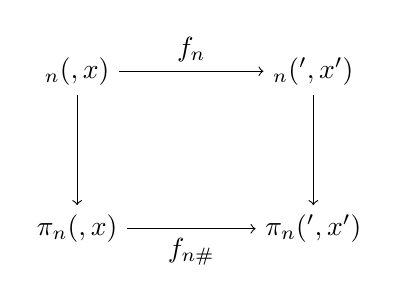
\begin{tikzpicture}[ auto]
      \node (A)  at (0,0) {$\PSLoops_n(\X,x)$};
      \node (B)  at (3,0) {$\PSLoops_n(\X',x')$};
      \node (C)  at (0,-2) {$\pi_n(\X,x)$};
      \node (D)  at (3,-2) {$\pi_n(\X',x')$};
      \draw[->] (A) to node {$f_n$} (B);
      \draw[->] (A) to node [swap] {$\comp$} (C);
      \draw[->] (B) to node {$\comp$} (D);
      \draw[->] (C) to node [swap] {$f_{n\#}$} (D);
    \end{tikzpicture}
    \end{center}
    For all $n \geq 0$, this whole construction defines a
    functor $\Pi_n$, from the category of pointed
    diffeological spaces to the category of groups, or
    pointed spaces,
    $$
      \Pi_n(\X,x) = \pi_n(\X,x) \qmbox{and}
      \Pi_n(f) = f_{n\#}.
      $$
    The main properties of $f_{n\#}$ are the following ones.

      \alinea{1.} If $f$ is a homotopy equivalence
      \art{The-homotopy-category}, then the $f_{n\#}$ are
      isomorphisms.
    
      \alinea{2.} If $\rho : \X \to \A$ is a deformation retraction
      \art{Retractions-and-deformation-retracts}, then the
      $\rho_{n\#}$ are isomorphisms from $\pi_n(\X,x)$ to
      $\pi_n(\A,x)$, where $x \in \A$.
    
      \alinea{3.} If $\X$ is contractible
      \art{Contractible-diffeological-spaces}, then $\pi_n(\X,x) = \set{0}$
      for all $n \geq 1$.
  \end{article} %% Higher-homotopy-groups
  
  \begin{proof}
    According to the recursive definition of the higher homotopy
    groups, it is enough to check that $f_{n\#}$ is a
    morphism for $n = 0$ and $n=1$. For
    $n = 0$, it is stated in 
    \art{Smooth-maps-and-connectedness}. For $n =1$, it is an
    immediate consequence of the fact that the image by $f$ of
    the concatenation of two paths $\gamma$ and
    $\gamma'$ is the concatenation of $f \circ \gamma $ and
    $f \circ \gamma'$.  
    Now, let us prove the following proposition. 
    
    \Lemma If $f : \X \to \X'$ is a homotopy equivalence, 
    then $f_1 : \Loops(\X,x) \to \Loops(\X',x')$, where $x' = f(x)$, is a
    homotopy equivalence.
    
    \alinea{}By definition, the map $f$ is a homotopy equivalence if
    there exists a smooth map $g : \X' \to \X$ such that $f$
    and $g$ are homotopic inverse one from each other, that is, $g
    \circ f$ 
    is homotopic to $\id_\X$ and $f \circ g$ is
    homotopic to $\id_{\X'}$. So, let $t \mapsto \xi_t$ be
    the homotopy from $\id_\X$ to $g \circ f$, that is, 
    $$ 
      \xi_0 = \id_\X \qmbox{and} \xi_1 = g \circ f.
      $$
    Let $y = g(x') = g \circ f (x)$. If $y = x$, then the
    path $s \mapsto [\ell \mapsto \xi_s \circ \ell]$ is
    obviously a homotopy from the identity of $\Loops(\X,x)$
    to $g_1 \circ f_1 = [\ell \mapsto g \circ f \circ \ell]$, and
    similarly for $f_1 \circ g_1$. We should conclude that
    $f_1$ and $g_1$ are homotopic inverse one from each other, but if
    $y \neq x$, we have to \guillemots{reconnect} $y$ to $x$. Now,
    let us recall that $\Loops(\X,x)$ and $\stLoops(\X,x)$ are
    homotopy equivalent, 
    \exref{Deformation-onto-stationary-paths}. So, we shall
    consider only stationary paths. Let $c = [t \mapsto
    \xi_{\lambda(t)}(x)]$, where $\lambda$ is the smashing
    function defined in \art{Homotopy-of-paths}, $c$ is a
    stationary path in $\X$ connecting $x$ to $y$.
    Now, let us define, for all $\ell' \in \stLoops(\X',x')$,
    $$
      \tilde g : \ell' \mapsto c \vee (g \circ \ell') \vee
      \bar c.
      $$
    Since $\ell'$ is stationary, $g \circ \ell'$ is
    stationary and $\tilde g(\ell')$ is a well defined loop in
    $\X$, based at $x$. So, $\tilde g$ is a smooth map from
    $\stLoops(\X',x')$ to $\stLoops(\X,x)$.
    Now, for every stationary loop $\ell$ in $\X$ based at
    $x$, $\xi_s \circ \ell$ is a stationary loop based at
    $\xi_s(x)$. Let us define now the stationary path $c_s =
    [t \mapsto \xi_{s\lambda(t)}(x)]$, connecting $x$ to
    $\xi_s(x)$. The map $s \mapsto c_s$ is a path in 
    $\stPaths(\X)$, and satisfies 
    $$
      c_s(0) = x, \quad c_s(1) = \xi_{s}(x), \quad c_0 = \bmx =
      [t \mapsto x], \qmbox{and} c_1 = c.
      $$
    Thus, for any $s$, for any $\ell \in \Paths(\X,x)$, $c_s$,
    $\xi_s(\ell)$ and $\bar c_s$ are juxtaposable, and their
    concatenation is a stationary path in $\X$ based at $x$.
    Then, let us define,  for all $\ell \in \stLoops(\X,x)$,
    \quad
    $$
      \Xi_s(\ell) = c_s \vee (\xi_s \circ \ell) \vee \bar c_s.
      $$
    The map $s \mapsto \Xi_s$ is a path in
    $\Cinfty(\stLoops(\X,x),\stLoops(\X,x))$ connecting
    $$
      \Xi_0 = [\ell \mapsto \bmx \vee \ell \vee \bmx]
      \qmbox{to} \Xi_1 = [\ell \mapsto c \vee (g \circ f \circ
      \ell) \vee \bar c] = \tilde g \circ f_1.
      $$
    Now, a slight adaptation of the part 2) of the proof of
    \art{The-Poincare-groupoid-and-fundamental-group} shows that the map $[\ell
    \mapsto \bmx \vee \ell \vee \bmx]$ is homotopic to the
    identity of $\st\Loops(\X,x)$. Hence, $\tilde g \circ f_1$
    is homotopic to the identity of $\st\Loops(\X,x)$. 
    We could prove, in the same way, that $f_1 \circ \tilde g$
    is homotopic to the identity of $\stPaths(\X',x')$.
    Therefore, $f_1$ is a homotopy equivalence and $f_{1\#}$
    is an isomorphism. By recurrence, we get that the
    $f_{n\#}$ are all isomorphisms. The case 1. is proved,
    the cases 2. and 3. are corollaries. 
  \end{proof}
  
  %%%%%%%%%%%%%%%%%%%%%%%%%%%%%%%%%%%%%%%%%%%%%%%%%%%%%%%%%%
  
  \section*{Relative Homotopy}
  \label{Relative-homotopy}
  
  \begin{sechead}
    This section describes the homotopy of a pair
    $(\X,\A)$, where $\X$ is a diffeological space and $\A$
    is a subspace of $\X$. We establish the short and 
    long exact sequences of
    the homotopy of the pair $(\X,\A)$, pointed at $a \in \A$, 
    which is a key
    ingredient of the exact homotopy sequence of the
    diffeological fiber bundles \art{Exact-homotopy-sequence-of-a-diffeological-fibration}.
  \end{sechead}
  
  \begin{article}\artlabel{The short homotopy sequence of a pair} 
    \addcontentsline{toc}{section}{\small\hspace{10pt} The short homotopy
    sequence of a pair} 
    \label{The-short-homotopy-sequence-of-a-pair}
    Let $\X$ be a
    diffeological space, let $\A$ be a subspace of $\X$, and
    let $a \in \A$. Let us recall
    \art{The-space-of-Paths-of-a-diffeological-space} that
    $$
    \Paths(\X,\A,a) = \set{ \gamma \in
    \Paths(\X) \mid \0(\gamma) \in \A \mbox{
    and } \1(\gamma) = a}.
    $$
    Let $\gamma$ and $\gamma'$ be two paths belonging 
    to $\Paths(\X,\A,a)$, a {\em homotopy
    from $\gamma$ to $\gamma'$, relative to $\A$, pointed at
    $a$} is a path in $\Paths(\X,\A,a)$, connecting $\gamma$
    to $\gamma'$. We shall also say an $(\A,a)$-relative
    homotopy from $\gamma$ to $\gamma'$. In the figure
    \ref{fig-relativeHomotopyOfAPair} the paths $\gamma$ and
    $\gamma'$ belong to $\Paths(\X,\A,a)$, with $\A = \A_1
    \cup \A_2$. The path $\gamma$ is $(\A,a)$-relatively
    homotopic to a loop in $\X$, but not $\gamma'$.
    %%###########
    \begin{figure}[tb]
      \centerline{\includegraphics{Figures-PDF/fig-relative-homotopy-II.pdf}}
      \caption{Relative homotopy of a pair.}
      \label{fig-relativeHomotopyOfAPair}
    \end{figure}
    %%###########
    Let us consider the map $\0 : \Paths(\X,\A,a)
    \to \A$ and the injection $i : \A \to \X$. They made
    up a two-terms sequence of smooth maps:
    $$
    \Paths(\X,\A,a) \rfl{\0} \A \rfl{i} \X.
    $$
    This sequence induces naturally the following two-terms
    sequence of morphisms of pointed spaces,
    $$
    (\Paths(\X,\A,a),\bma) \rfl{\0} (\A,a) \rfl{i}
    (\X,a),
    $$
    where $\bma = [t \mapsto a]$. Then, this sequence
    induces a two-terms sequence on the space of components
    \art{Smooth-maps-and-connectedness},
    \begin{equation}
      \renewcommand{\theequation}{$\heartsuit$}
      \pi_0(\Paths(\X,\A,a),\bma) \rfl{\0_\#}
      \pi_0(\A,a) \rfl{i_\#} \pi_0(\X,a).
    \end{equation}
    
    \alinea{1.} $\ker(i_\#)$ --- The {\em
    kernel} of $i_\#$ is
    the subset of components of $\A$, contained in the
    component of $\X$ containing $a$.
    
    \alinea{2.} $\Val(\0_\#)$ --- The {\em values} of
    $\0_\#$ are the components of $\A$,
    containing the initial points of the paths in $\X$ starting in
    $\A$ and ending at $a$. In other words, the subset of
    the components of $\A$ which can be connected, through $\X$,
    to $a$.
    Now, it is clear that any component of $\A$ which can be
    connected to $a$ by a path in $\X$ is included in the
    component of $\X$ containing $a$. Conversely, every
    component of $\A$ included in the component of $\X$
    containing $a$ can be connected to $a$ by a path in
    $\X$, starting in $\A$. So, we get the equality,
    $$
    \ker(i_\#) = \Val(\0_\#).
    $$
    Now, let us consider the inclusion of the triple
    $(\X,a,a)$ into $(\X,\A,a)$. It induces an injection,
    denoted by $j$, on the space of paths,
    $$
    \Paths(\X,a,a) = \Loops(\X,a) \rfl{j} \Paths(\X,\A,a).
    $$
    This injection projects, on the space of components, into a
    morphism of pointed spaces,
    \begin{equation}
      \renewcommand{\theequation}{$\diamondsuit$}
      \pi_0(\Loops(\X,a),\bma) \rfl{j_\#}
      \pi_0(\Paths(\X,\A,a), \bma).
    \end{equation}
    Now, the concatenation of $(\diamondsuit)$ to the two-terms 
    sequence $(\heartsuit)$ gives a three terms sequence
    of morphisms of pointed spaces,
    \begin{equation} \renewcommand{\theequation}{$\spadesuit$}
    \pi_0(\Loops(\X,a),\bma)  \rfl{j_\#}  \pi_0(\Paths(\X,\A,a),\bma))  \rfl{\0_\#}  \pi_0(\A,a)  \rfl{i_\#}
    \pi_0(\X,a).
    \end{equation}
    Let us call, by abuse of language, {\em first group of
    homotopy of $\X$, relative to $\A$, pointed at $a$}, the
    pointed space denoted by $\pi_1(\X,\A,a)$, and defined by
    $$
    \pi_1(\X,\A,a) = \pi_0(\Paths(\X,\A,a), \bma).
    $$
    Since, by definition, $\pi_0(\Loops(\X,a),\bma) =
    \pi_1(\X,a)$ \art{The-Poincare-groupoid-and-fundamental-group} --- regarded
    as pointed space --- the sequence of morphisms
    $(\spadesuit)$ rewrites,
    \begin{equation}
      \renewcommand{\theequation}{$\clubsuit$}
      \pi_1(\X,a) \rfl{j_\#} 
      \pi_1(\X,\A,a) \rfl{\0_\#}
      \pi_0(\A,a) \rfl{i_\#} \pi_0(\X,a).
    \end{equation}
    This sequence is called the {\em short sequence
    of the relative homotopy of the pair $(\X,\A)$, at the
    point $a$}. We have seen that $\ker(i_\#) =
    \Val(\0_\#)$, moreover:
    $$
    \ker(\0_\#) = \Val(j_\#).
    $$
    
    \alinea{3.} $\ker(\0_\#)$ --- The kernel of
    $\0_\#$ is the set of the components of
    $\Paths(\X,\A,a)$ whose initial point belongs to the
    component of $\A$ containing $a$.
    
    \alinea{4.} $\Val(j_\#)$ --- The values of
    $j_\#$ are the components of the $\gamma \in \Paths(\X,\A,a)$ 
    which are $(\A,a)$-relatively homotopic
    to some loops in $\X$, based at $a$. 
    
    \alinea{}In short, the relative homotopy sequence of the pair $(\X,\A)$,
    at the point $a$, is exact.
  \end{article} %% The-short-homotopy-sequence-of-a-pair
  
  \begin{proof}
    We need only check that $\ker(\0_\#) =
    \Val(j_\#)$. Let us recall that, on the one hand,
    $\ker(\0_\#)$ is made up of the components of
    $\Paths(\X,\A,a)$ whose initial point belongs to the
    same component of $\A$, containing $a$. On the other hand, $\Val(j_\#)$
    is the set of the components of paths $\gamma \in
    \Paths(\X,\A,a)$ which are $(\A,a)$-relatively homotopic
    to some loops in $\X$, based at $a$.
    
    \alinea{1.} $\Val(j_\#) \subset \ker(\0_\#)$. If a path
    $\gamma$ is $(\A,a)$-relatively homotopic to some loop in
    $\X$ based at $a$, its initial point is connected, in
    $\A$, to $a$, and belongs to the same component of
    $\A$ containing $a$.
    
    \alinea{2.} $\ker(\0_\#) \subset \Val(j_\#)$.  Let us
    consider a component of $\A$ contained in the
    same component of $\X$ containing $a$. Let $\gamma$ be a
    stationary path in $\X$, beginning in $\A$ and ending at
    $a$ such that its beginning belongs to the component of
    $\A$ containing $a$. Let $\gamma(0) = x$. Since $x$ and
    $a$ belong to the same component of $\A$, there exists a
    stationary path $c$ in $\A$ connecting $a$ to $x$
    \fig{fig-relativeHomotopyOfAPair}. Let $\xi(s) = [t
    \mapsto c(s + (1-s)\lambda(t))]$, where $\lambda$ is the
    smashing function described in
    \fig{fig-smashing-function}. Thus, $\xi$ belongs to
    $\Paths(\Paths(\X,\A,a))$ \art{Relative-homotopy} and
    $\xi(s)(1) = c(1) = x = \gamma(0)$. So, $\sigma(s)
    = \xi(s) \vee \gamma$ is a homotopy connecting $(c
    \circ \lambda) \vee \gamma \in \Loops(\X,a)$ to $\bmx
    \vee \gamma$, which is homotopic to $\gamma$. Therefore
    $\gamma$ is $(\A,a)$-relatively homotopic to a loop in
    $\X$, based at $a$. 
  \end{proof}
  
  \begin{article}\artlabel{The long homotopy sequence of a pair} 
    \addcontentsline{toc}{section}{\small\hspace{10pt} The long homotopy
    sequence of a pair} 
    \label{The-long-homotopy-sequence-of-a-pair}
    Let $\X$ be a
    diffeological space, let $\A$ be a subspace of $\X$, and
    let $a \in \A$. Let us denote again by $i$
    the natural induction $i : \Loops(\A,a) \to
    \Loops(\X,a)$. There is no ambiguity with the injection
    $i$ of \art{The-short-homotopy-sequence-of-a-pair}, since
    the spaces involved are not the same. Then, let us
    consider the two terms sequence of smooth maps
    $$
      \Paths(\Loops(\X,a),\Loops(\A,a), \bma) \rfl{\0}
      \Loops(\A,a) \rfl{i} \Loops(\X,a).
      $$
    Or, if we prefer, by denoting
    $$
      \X_1 = \Loops(\X,a), \quad \A_1 = \Loops(\A,a) 
      \qmbox{and} a_1 = [t \mapsto a],
      $$
    the above two terms sequence of smooth maps writes
    $$
      \Paths(\X_1,\A_1, a_1) \rfl{\0}
      \A_1 \rfl{i} \X_1.
      $$
    We can then apply the construction of
    \art{The-short-homotopy-sequence-of-a-pair} and get the
    short sequence of relative homotopy of the pair
    $(\X_1,\A_1)$, at the point $a_1$. 
    Let us denote again by
    $j$ the natural induction from $\Loops(\X_1,a_1)$ to
    $\Paths(\X_1,\A_1,a_1)$. Thus, we have,
    \begin{equation}
      \renewcommand{\theequation}{$\diamondsuit$}
      \pi_1(\X_1,a_1) \rfl{j_\#} 
      \pi_1(\X_1,\A_1,a) \rfl{\0_\#}
      \pi_0(\A_1,a_1) \rfl{i_\#} \pi_0(\X_1,a_1).
    \end{equation}
    Let us define the second group of relative homotopy of the
    pair $(\X,\A)$, at the point $a$, by
    $$
      \pi_2(\X,\A,a) =
      \pi_1(\X_1,\A_1,a_1) = \pi_0(\Paths(\X_1,\A_1,a_1),a_1).
      $$
    So, the short exact sequence
    $(\diamondsuit)$ writes now
    \begin{equation}
      \renewcommand{\theequation}{$\heartsuit$}
      \pi_2(\X,a) \rfl{j_\#} 
      \pi_2(\X,\A,a) \rfl{\0_\#}
      \pi_1(\A,a) \rfl{i_\#} \pi_1(\X,a).
    \end{equation}
    But the right term
    $\pi_1(\X,a) = \pi_0(\X_1,a_1)$ is just
    $\pi_0(\Loops(\X,a),\bma)$, that is, $\pi_1(\X,a)$,
    regarded as a pointed space. It is also the left term of
    the relative homotopy sequence of the pair $(\X,\A)$ at
    the point $a$,
    \art{The-short-homotopy-sequence-of-a-pair}. Let us
    connect the right term of the short homotopy sequences
    relative to the pair $(\X_1,\A_1)$, to the left term of
    the short homotopy sequences
    relative to the pair $(\X,\A)$. We get,
    $$
      \cdots \
      \pi_2(\X,\A,a) \rfl{\0_\#}
      \pi_1(\A,a) \rfl{i_\#}
      \pi_1(\X,a) \rfl{j_\#} 
      \pi_1(\X,\A,a) \rfl{\0_\#}
      \pi_0(\A,a) \ \cdots
      $$
    Then, let us describe the connection of the morphisms
    of these two relative homotopy sequences at the junction
    $\pi_1(\X,a)$.
    
    \alinea{1.} $\ker(j_\# : \pi_1(\X,a) \to
    \pi_1(\X,\A,a))$ --- This kernel is the set of classes of loops
    of $\X$ based at $a$ which can be connected, relatively
    to $(\A,a)$, to the constant loop $\bma$.
    
    \alinea{2.} $\Val(i_\# : \pi_1(\A,a) \to
    \pi_1(\X,a))$ --- This is the set of classes
    of loops in $\X$, based at $a$, which are fixed-ends
    homotopic to a loop in $\A$. 
    
    \alinea{}Now, if a loop in $\X$, based at $a$,
    can be smoothly deformed into a loop contained in $\A$,
    then it can be retracted relatively to $\A$ into the
    constant loop $\bma$. Conversely, if a loop of $\X$, based
    at $a$, is connected relatively to $(\A,a)$ to the constant loop $\bma$,
    then it is fixed-ends homotopic to a
    loop in $\A$. In other words:
    $$
      \ker(j_\# : \pi_1(\X,a) \to
      \pi_1(\X,\A,a)) = \Val(i_\# : \pi_1(\A,a) \to
      \pi_1(\X,a)).
      $$
    Thus, the connection of the two short exact relative
    homotopy sequences is exact. 
    Now, let us define the {\em
    higher relative homotopy groups} of the pair $(\X,\A)$ 
    at the point $a$ by recurrence. 
    Let us remark first that the inclusion 
    $i : \A \to \X$ induces an inclusion 
    $i_n : \Loops_n(\A,a) \to \Loops_n(\X,a)$ 
    \art{Higher-homotopy-groups}. Then, we can define
    $$
      \Paths_{n+1}(\X,\A,a) = \Paths(\Loops_n(\X,a),\Loops_n(\A,a), \bma_n),
      $$
    for every integer $n$, and this gives the higher
    relative homotopy groups    
    \begin{eqnarray*}
      \pi_{n+1}(\X,\A,a) &  = & \pi_0(\Paths_{n+1}(\X,\A,a),\bma_n) \\
      & = & \pi_1(\Loops_n(\X,a),\Loops_n(\A,a), \bma_n).
    \end{eqnarray*}
    Now, we can iterate the above connection of short relative
    homotopy sequences for each degree $n+1 \to n$, and we get
    {\em the long exact relative homotopy sequence of the pair
    $(\X,\A)$, at the point $a$}. 
    \begin{equation}
      \renewcommand{\theequation}{$\clubsuit$}
      \left.
      \begin{array}{r@{\hspace{-2pt}}c@{\hspace{-2pt}}c@{\hspace{-2pt}}c@{\hspace{-2pt}}c@{\hspace{-2pt}}c@{\hspace{-2pt}}c@{\hspace{0pt}}l@{\hspace{-2pt}}l}
        \cdots \rfl{i_\#} &  \pi_n(\X,a) & \rfl{j_\#} & \pi_n(\X,\A,a) & \rfl{\0_\#} & \pi_{n-1}(\A,a) & \rfl{i_\#} & \pi_{n-1}(\X,a) \cdots\,
        \\
        \vspace{-5pt} 
        \\
        \cdots \rfl{i_\#} &  \pi_1(\X,a) & \rfl{j_\#} & \pi_1(\X,\A,a) & \rfl{\0_\#} & \pi_0(\A,a)     & \rfl{i_\#} & \pi_0(\X,a).  
      \end{array}
      \right\}
    \end{equation}
  \end{article} %% The-long-homotopy-sequence-of-a-pair
  
  \begin{proof}
    We need only check that $\ker(j_\# : \pi_1(\X,a) \to
    \pi_1(\X,\A,a))$ is equal to $\Val(i_\# : \pi_1(\A,a) \to
    \pi_1(\X,a))$. Let us recall that 
    $\ker(j_\#)$ is made up of the loops
    of $\X$ based at $a$ which can be connected, relatively
    to $(\A,a)$, to the constant loop $\bma$, and
    $\Val(i_\#)$ is the subset of the
    classes of loops in $\X$, based at $a$, which are
    fixed-ends homotopic to a loop in $\A$. 
    
    \alinea{1.} $\ker(j_\#) \subset \Val(i_\#)$.
    Let $\ell$ be a loop in $\X$, based at $a$,
    $(\A,a)$-relatively homotopic to the constant loop
    $\bma$. Let $\gamma$ be the homotopy. So, for all $s \in
    \RR$,
    $$
    \gamma(0) = \ell, \quad \gamma(1) = \bma, \quad
    \gamma(s)(0) \in \A \qmbox{and} \gamma(s)(1) = a.
    $$
    The properties of $\gamma$ are schematized by the figure
    \ref{fig-relativeHomotopyOfLoop}. 
    %%###########
    \begin{figure}[tb]
      \centerline{\includegraphics{Figures-PDF/fig-relative-homotopy-III.pdf}}
      \caption{A relative homotopy of a loop to the constant loop.}
      \label{fig-relativeHomotopyOfLoop}
    \end{figure}
    %%###########
    Let us consider a line
    of $\RR^2$, turning around the origin, its intersection
    with the cube describes a homotopy connecting $\ell$ to
    $\gamma_{t=0} \in \Loops(\A,a)$. More precisely, let us
    consider first the path $\gamma' : s \mapsto [t \mapsto \gamma(t)(st)]$ 
    in $\Loops(\X,a)$.
    The path $\gamma'$ connects $\ell$ to $[t \mapsto
    \gamma(t)(t)]$. Then, let us consider the path 
    $\gamma'' : s \mapsto [t \mapsto \gamma((1-s)t)(t)]$
    in $\Loops(\X,a)$.
    The path $\gamma''$ connects $[t \mapsto
    \gamma(t)(t)]$ to $\gamma_{s=0} \in \Loops(\A,a)$.
    Therefore, $\ell$ is $(\A,a)$-relatively homotopic to a
    loop in $\A$, based at $a$.
    
    \alinea{2.} $\Val(i_\#) \subset \ker(j_\#)$. Let $\comp(\gamma) \in
    \Val(i_\#)$. We can choose 
    $\gamma \in \Loops(\A,a)$. The path $\xi : s \mapsto [t \mapsto \gamma(s + (1-s)t)]$
    is a $(\A,a)$-relative homotopy connecting $\gamma$ to
    the constant loop $\bma$.
  \end{proof}
  
  \begin{article}\artlabel{Another look at relative homotopy}  
    \addcontentsline{toc}{section}{\small\hspace{10pt} Another look at
    relative homotopy}
    \label{Another-look-at-relative-homotopy} Let
    $\X$ be a diffeological space, let $\A$ be a subspace of
    $\X$, and let $a \in \A$. We shall give another
    description of the relative homotopy groups
    $\pi_n(\X,\A,a)$. Let us begin by $n = 2$, then
    $\pi_2(\X,\A,a) = \pi_1(\Loops(\X,a),\Loops(\A,a),
    \bma)$. Let 
    $$
    f \in \Paths(\Loops(\X,a),\Loops(\A,a), \bma).
    $$ 
    Thus, for all $(s,t) \in \RR^2$,
    $$
    f(0) \in
    \Loops(\A,a), \quad f(1)(t) = a, \qmbox{and}
    f(s)(0) = f(s)(1) = a.
    $$
    We identify $f$ with a smooth plot $f : \RR^2 \to
    \X$ by $f(s,t) = f(s)(t)$, the properties of $f$ are
    described by \fig{fig-relLoops2}.
    %%###########
    \begin{figure}[tb]
      \centerline{\includegraphics{Figures-PDF/fig-relative-homotopy-I.pdf}}
      \caption{$f$ belonging to
      $\relativeLoops_2(\X,\A,a)$.}
      \label{fig-relLoops2}
    \end{figure}
    %%###########
    Then, let us permute the
    variables $t$ and $s$, let 
    $$
    \tilde f (t)(s) = f(s)(t).
    $$
    Now, $\tilde f$ satisfies, for all $t \in \RR$
    $$
    \tilde f(t) \in \Paths(\X,\A,a), \qmbox{and} \tilde f(0)
    = \tilde f(1) = \bma.
    $$
    Thus, $\tilde f \in
    \Loops(\Paths(\X,\A,a),\bma)$. Now, since $(t,s) \mapsto
    (s,t)$ is a diffeomorphism, $f \mapsto \tilde f$ is a
    diffeomorphism. More generally, 
    $$
    f \in \Paths(\Loops_n(\X,a), \Loops_n(\A,a),\bma_n), \qmbox{for all} n \geq 1.
    $$
    Let $\tilde f$ be defined by
    $$
    \tilde
    f(t_0)(t_1)\cdots(t_n) = f(t_1)\cdots(t_n)(t_0).
    $$
    Then, $\tilde f$ belongs to $\Loops_n(\Paths(\X,\A,a), \bma)$, 
    and the map $f \mapsto \tilde f$ is a
    diffeomorphism. So, thanks to this identification, we
    get,  
    $$
    \pi_{n+1}(\X,\A,a) = \pi_n(\Paths(\X,\A,a), \bma), \qmbox{for all} n \geq 1.
    $$
    Therefore, the relative homotopy groups $\pi_n(\X,\A,a)$
    are pointed spaces for $n = 1$, groups for $n=2$, Abelian
    groups for $n \geq 3$. Moreover, the morphisms of the
    long exact homotopy sequence of the pair $(\X,\A)$, at
    the point $a$,
    \art{The-long-homotopy-sequence-of-a-pair}~$(\clubsuit)$,
    are group morphisms wherever it makes sense. Indeed, the
    operator $\0_\#$ acts on the first variable of the
    path of loops, while the group acts on the last one. 
  \end{article} %% Another-look-at-relative-homotopy
  
  %%%%%%%%%%%%%%%%%%%%%%%%%%%%%%%%%%%%%%%%%%%%%%%%%%%%%%%%%%
  %
  %   Exercises
  %
  %%%%%%%%%%%%%%%%%%%%%%%%%%%%%%%%%%%%%%%%%%%%%%%%%%%%%%%%%%
  
  \Exercise
  
  \begin{exercise}[Homotopy of loops spaces]  
    \label{Homotopy-of-loops-spaces}
    Let $\X$ be a connected diffeological space, $\pi_0(\X) = \{\X\}$. 
    Show that $\pi_0(\Loops(\X))$ is equivalent to the set of conjugacy classes 
    of $\pi_1(\X,x)$ where $x$ is any given point in $\X$. 
    Comment the homotopy of $\Loops(\X)$ relatively to $\Loops(\X,x)$.
  \end{exercise} %% Homotopy-of-loops-spaces
